\documentclass[aps,prl,reprint,superscriptaddress,longbibliography]{revtex4-2}
\usepackage{amsmath,amssymb,bm,graphicx,hyperref}
\hypersetup{colorlinks=true,linkcolor=blue,citecolor=blue,urlcolor=blue}
\newcommand{\Tr}{\operatorname{Tr}}
\newcommand{\Var}{\operatorname{Var}}
\newcommand{\Wd}{W_{\mathrm{diss}}}
\newcommand{\dd}{\mathrm{d}}
\begin{document}
\title{Rare work costs under bounded-action quantum confinement control}
\author{R. Arun Chandru}
\email{arun.chandru@gmail.com}
\date{October 6, 2026}
\begin{abstract}
Preserving almost every energy-level label need not suppress the energetic fluctuations of a controlled quantum system. We establish this distinction for a thermal particle confined by a finite wall whose height is changed by a finite factor. As the penetration length $r$ vanishes, the label-changing probability is of order $r^2$, whereas events of probability $r^3$ at energies of order $r^{-2}$ carry the leading dissipated work and a divergent work variance. A boundary-source construction determines the complete weighted rare-event law. Positive lower bounds survive uniformly over all wall-height protocols with bounded integrated action, including protocols that depend on $r$. The obstruction is a non-square-integrable endpoint displacement that a bounded-norm dynamical correction cannot cancel. For fixed protocols, finitely many final-energy bands recover arbitrarily much of the leading dissipative relative entropy, while energy-basis coherence is subleading. The results cover sharp walls and fixed smooth profiles, and a continuum interval certificate gives a finite-height work bound.
\end{abstract}
\maketitle

Quantum control is often assessed by the probability of preparing a target state or preserving selected level populations. Work statistics ask a different question: what energy is carried by the small part of the state that misses the target? The distinction becomes consequential when confinement creates an increasing energy scale. A small error probability can then conceal a large second moment, and a low-energy effective boundary condition need not describe the energetic cost of changing the physical wall.

Work distributions and their thermodynamic interpretation are well studied subjects \cite{Talkner,Campisi}. Exactly solvable local quenches exhibit endpoint-dependent work edges \cite{Smacchia}; quantum work distributions have nonclassical tails \cite{Jarzynski}, and sudden changes of ideal walls can produce singular energy moments \cite{Aslangul}. Rare transitions also matter in rapidly moving quantum pistons \cite{Quan}. Generalized linear response treats complete work statistics for weak perturbations \cite{Guarnieri}, while rapid-driving expansions address dissipation and fluctuation control \cite{Rolandi}. Recent boundary-conformal results give a saturable work-fluctuation speed limit in a specified weak-driving regime \cite{Xia}. These results motivate a finite-amplitude question retaining the microscopic wall: can pulse shaping remove its rare energetic cost while preserving almost all level labels?

Here we resolve this question for a precise thermal confinement family and a physically defined control budget. Our contribution is the combination of an actual finite-wall source law, control-uniform lower bounds, and a final-energy certificate of the leading dissipation. The bounds concern integrated wall-height action, not minimum duration or a proved attainable optimal protocol. Standard control estimates \cite{BoussaidCost,BoussaidWeak} and entropy identities \cite{Deffner,Francica} enter explicitly; the singular boundary source supplies the model-specific obstruction.

\emph{Finite walls and the control resource.---}
Let $E_0=\hbar^2/(2mL^2)$, measure lengths in $L$ and times in $\hbar/E_0$, and put $\theta=\beta E_0>0$. A single particle occupies $(0,1+b)$, with Dirichlet conditions only at its two outer endpoints. Its dimensionless Hamiltonian is
\begin{equation}
 K_r(t)=-\partial_y^2+r^{-2}\gamma_r(t/\tau_r)M_r(y),
 \qquad \tau_r=\eta_r r^2. \label{eq:model}
\end{equation}
Here $b>0$, $\gamma_r(0)=1$, and $\gamma_r(1)=g>0$, with $g\ne1$. Each path is positive and absolutely continuous. The sharp wall is $M_r=\mathbf1_{(1,1+b)}$. We also allow $M_r(y)=V((y-1)/r)$ for any fixed real smooth profile with $0\le V\le1$, $V=0$ on $(-\infty,0]$, and $V=1$ on $[a,\infty)$, where $a>0$ is fixed. Spatial monotonicity is unnecessary. The smooth transition width is $arL$; it is not held fixed in laboratory units as $r\to0$.

The initial state is the complete Gibbs state $\rho_{i,r}=e^{-\theta K_{i,r}}/Z_{i,r}$, including all exterior and above-barrier modes. The evolution is isolated and unitary. If $e_n^i,e_m^f$ are the ordered endpoint eigenvalues, two energy measurements give probabilities $p_n|\langle\phi_m^f,\mathcal U_r\phi_n^i\rangle|^2$ and dimensionless work $W=e_m^f-e_n^i$. We write $\Wd=\mathbb EW-\Delta\mathcal F$, with $\Delta\mathcal F=-\theta^{-1}\log(Z_f/Z_i)$. This dissipated work is not heat transferred to a bath during the protocol.

The common resource bound is
\begin{equation}
 \Lambda_r=\eta_r\int_0^1|\gamma_r(s)-1|\,\dd s\le\Lambda,\qquad0<\Lambda<\infty.
 \label{eq:action}
\end{equation}
For physical wall height $B(t_{\rm phys})$, this equals $\hbar^{-1}\int|B(t_{\rm phys})-B_i|\,\dd t_{\rm phys}$. The class $\mathcal C_r(\Lambda)$ permits $r$-dependent paths and durations without a common derivative, peak-height, or switch-count bound. Waiting at the initial height costs no action. Auxiliary potentials and changes of spatial profile are not included.

\emph{Typical outcomes and rare energetic events.---}
The endpoints determine a scattering-length difference $c=\ell_1-\ell_g\ne0$. The decaying zero-energy solution $w_q$ of $(-\partial_z^2+qV)w_q=0$ is normalized by $w_q'(0)=-1$ and extended as $w_q(z)=\ell_q-z$ for $z<0$. For a step, $\ell_q=q^{-1/2}$. Let
\begin{equation}
 U_D=\frac{\sum_{n\ge1}(n\pi)^2e^{-\theta(n\pi)^2}}
 {\sum_{n\ge1}e^{-\theta(n\pi)^2}}.
 \label{eq:ud}
\end{equation}
Uniformly on $\mathcal C_r(\Lambda)$, the probability of changing the ordered energy label satisfies
\begin{equation}
 \Pr(m\ne n)=c^2\left(\frac{U_D}{3}+\frac14\right)r^2+o(r^2).
 \label{eq:label}
\end{equation}
The familiar square-well dilation susceptibility \cite{Pizio} provides the coefficient; the new issue is what this nearly population-preserving behavior leaves uncontrolled.

Fix, for the moment, one path $\gamma$, one scaled duration $\eta$, and one spatial profile. A localized full-line source $G$ determines the positive measure
\begin{equation}
 \dd\nu(E)=2U_D E^{-2}\dd\mu_G(E),\quad
 \mu_G(S)=\langle G,\mathbf1_S(h_g)G\rangle,
 \label{eq:nu}
\end{equation}
where $h_g=-\partial_z^2+gV$. On positive energy windows separated from zero,
\begin{equation}
 r^{-3}\Pr(r^2W\in\dd E)\longrightarrow\dd\nu(E).
 \label{eq:rare}
\end{equation}
More importantly, the energy-weighted limits close with no hidden contribution at zero or infinity:
\begin{align}
 \frac{\Wd}{r}&\longrightarrow C_D=2U_D\int E^{-1}\dd\mu_G(E)>0,\label{eq:mean}\\
 r\Var W&\longrightarrow C_V=2U_D\|G\|^2>0.\label{eq:variance}
\end{align}
Thus the order-$r^3$ sector at physical energies $E_0/r^2$ controls an order-$r$ mean cost and an order-$r^{-1}$ variance. The larger order-$r^2$ label-changing sector in Eq.~\eqref{eq:label} does not supply these weighted limits. The absolute mean cost tends to zero; the fluctuation scale grows.

The source is constructive rather than a formal evolution of a nonnormalizable state. Put $f=Vw_1$, let $\mathcal V(s,u)$ propagate $h_{\gamma(s)}$ with $i\partial_s\mathcal V=\eta h_{\gamma(s)}\mathcal V$, and define the square-integrable correction
\begin{align}
 \zeta(s)&=-i\eta\int_0^s\mathcal V(s,u)(\gamma(u)-1)f\,\dd u,\nonumber\\
 G&=\int_0^1\mathcal V(1,s)\gamma'(s)[f+V\zeta(s)]\,\dd s.
 \label{eq:source}
\end{align}
At finite $r$, an exact differentiated-propagator identity relates each work-weighted transition amplitude to its corresponding localized source. Strong convergence on expanding intervals and Gaussian Gibbs-tail bounds then yield Eq.~\eqref{eq:rare} and its second moment. A separate homogeneous-energy identity proves the inverse moment in Eq.~\eqref{eq:mean}; it is not obtained by inserting an unbounded test into weak convergence. These steps and the complete first-moment remainder are derived in the Supplemental Material \cite{SM}.

\emph{Why bounded-action pulse shaping cannot remove the cost.---}
The key identity is
\begin{equation}
 G=(g-1)f+h_g\zeta(1)=h_g[k+\zeta(1)],\qquad k=w_1-w_g.
 \label{eq:affine}
\end{equation}
Although $k$ has finite homogeneous energy, it equals the nonzero constant $c$ on the whole left half-line and is not in $L^2$. In contrast, unitarity gives $\|\zeta(1)\|\le\Lambda\|f\|$. Finite-action control therefore cannot cancel the endpoint displacement. This is an infrared obstruction in the boundary coordinate, whose physical manifestation is the rare high-energy sector of the finite box.

To quantify it, enlarge the accessible dynamical corrections to the entire $L^2$ ball of radius $R=\Lambda\|f\|$. Define
\begin{align}
 D_{V,g}(R)&=\inf_{\|v\|\le R}\|(g-1)h_g^{-1/2}f+h_g^{1/2}v\|^2,\nonumber\\
 \mathcal V_{V,g}(R)&=\inf_{\|v\|\le R}\|(g-1)f+h_gv\|^2.
 \label{eq:relax}
\end{align}
The infima are over the appropriate form and operator domains, respectively. Spectral completion of squares, a norm-constrained quadratic minimization \cite{MoreSorensen}, reduces each to a one-parameter integral against the spectral measure of $f$. Both are strictly positive for every finite $R$. Figure~\ref{fig:bounds} illustrates the step-wall envelopes; they are lower bounds from an enlarged class, not reachable optimal controls.

Crucially, the same mechanism holds uniformly \emph{before} selecting a limiting protocol:
\begin{align}
 \liminf_{r\to0}\inf_{\mathcal C_r(\Lambda)}\frac{\Wd}{r}
 &\ge2U_D D_{V,g}(\Lambda\|f\|)>0,\nonumber\\
 \liminf_{r\to0}\inf_{\mathcal C_r(\Lambda)}r\Var W
 &\ge2U_D\mathcal V_{V,g}(\Lambda\|f\|)>0.
 \label{eq:uniform}
\end{align}
This does not follow by interchanging an infimum with the fixed-path limits. At finite $r$, Duhamel's formula bounds the dynamical correction, and a shifted affine source identity retains the initial eigenenergy. Bounded spectral multipliers supply the lower estimates. For the mean, the negative excess relative to same-label transport is uniformly $O(r^2)$. For the variance, the uniform $O(r^2)$ off-label probability and the thermally bounded $O(r)$ same-label shifts control centering. Only the resulting static endpoint operators are passed to the limit. Consequently rapidly varying or long-duration paths cannot evade Eq.~\eqref{eq:uniform} merely by depending on $r$.

\begin{figure}[t]
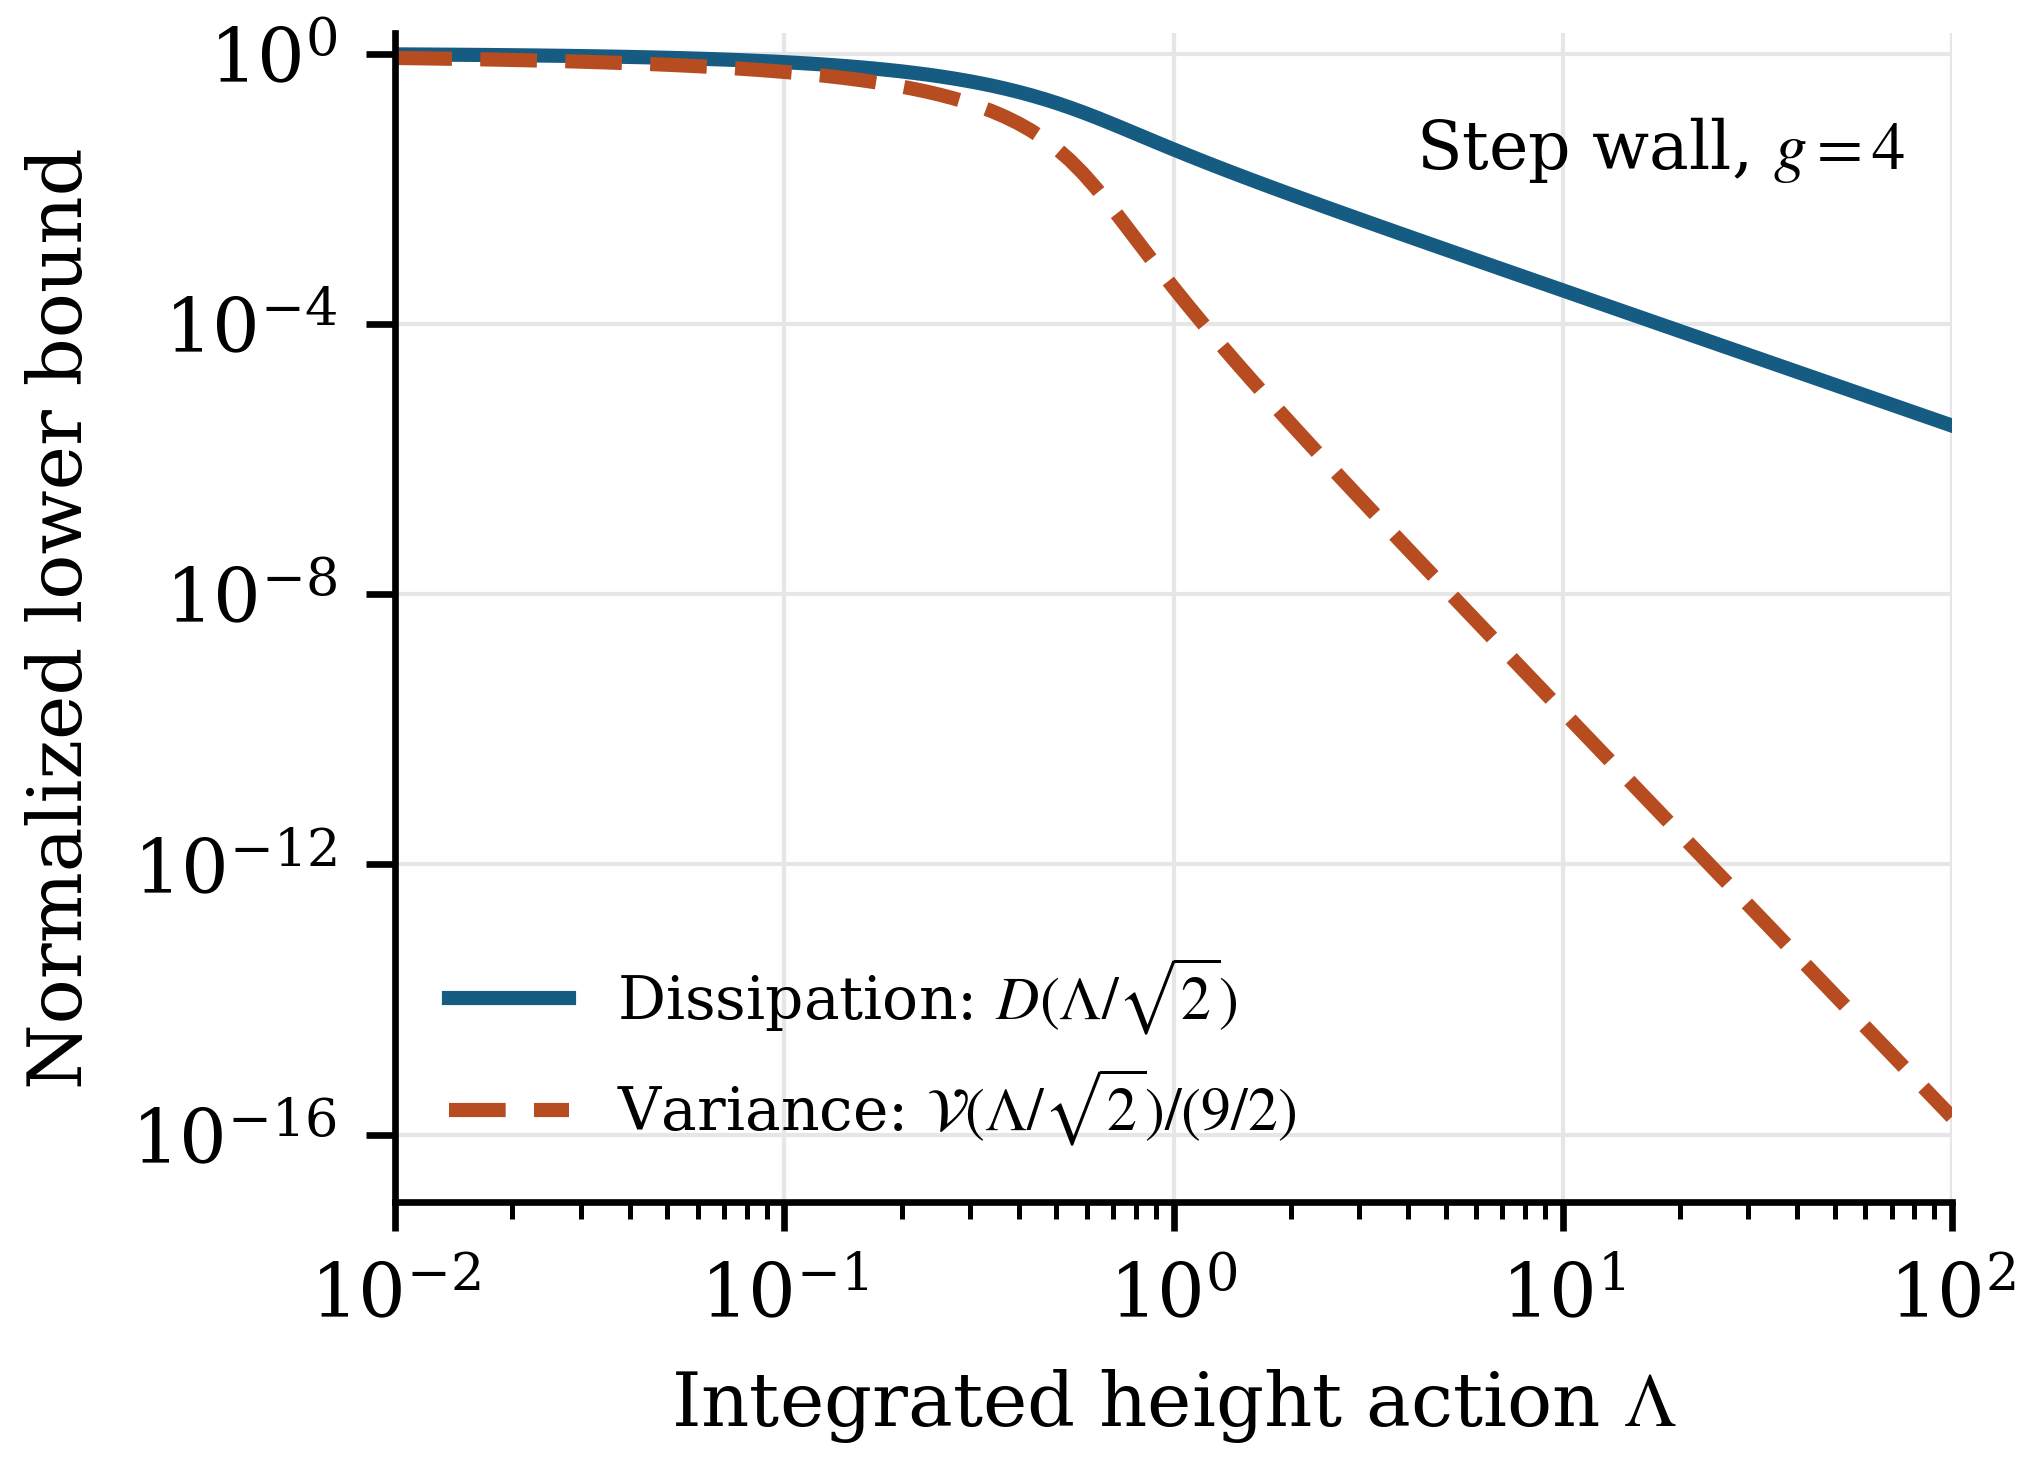
\includegraphics[width=\columnwidth]{control_bounds.png}
\caption{Control-uniform coefficient bounds for a sharp wall with endpoint ratio $g=4$. The curves are $D_{V,4}(\Lambda/\sqrt2)$ and $\mathcal V_{V,4}(\Lambda/\sqrt2)$, normalized by their zero-radius values, $1$ and $9/2$, respectively. These are computed from the exact spectral minimizations, not by optimizing waveforms. They stay positive at every finite action. Their large-action exponents differ, $\Lambda^{-2}$ and $\Lambda^{-6}$; this is a property of the relaxed bounds, not an asserted attainable tradeoff.}
\label{fig:bounds}
\end{figure}

\emph{Final energy counts retain the leading thermodynamic information.---}
An initial energy measurement is unnecessary for the following observable consequence: the initial Gibbs state is already energy diagonal. Write $F$ for the actual final-energy outcome of $\rho_r=\mathcal U_r\rho_{i,r}\mathcal U_r^*$ and $\sigma_r=e^{-\theta K_f}/Z_f$. For fixed path, duration and profile, the final distribution has the same rare measure $\nu$ and $r\Var F\to C_V$. This transfer controls the full thermal initial-energy moments, rather than setting the initial energy to zero in rare events.

Measure a finite collection of disjoint scaled-energy bands $J_j=[a_j,b_j)\subset(0,\infty)$ and the complementary outcome. Let $p_{j,r},q_{j,r}$ be the outcome probabilities in $\rho_r,\sigma_r$. The standard Gibbs identity and data processing give \cite{Deffner,Rubino}
\begin{equation}
 D_{\rm cat}(p_r\Vert q_r)\le D(\rho_r\Vert\sigma_r)=\theta\Wd.
 \label{eq:entropy}
\end{equation}
The rare probabilities obey $p_{j,r}=r^3\nu(J_j)+o(r^3)$, whereas a heat-trace bound gives $q_{j,r}\le C_jr^{-1}\exp(-\theta a_j/r^2)$. Therefore
\begin{equation}
 \liminf_{r\to0}\frac{D_{\rm cat}(p_r\Vert q_r)}{\theta r}
 \ge\sum_j a_j\nu(J_j).
 \label{eq:bins}
\end{equation}
The entropy of the outcome distribution is only $O(r^3|\log r|)$. Finite lower sums recover arbitrarily much of $C_D=\int E\,\dd\nu(E)$: for each $\epsilon>0$, finitely many bands chosen before $r\to0$ make the ratio in Eq.~\eqref{eq:entropy} at least $1-\epsilon$ in the lower limit. The chosen bands may depend on the fixed protocol and $\epsilon$; a common finite instrument for all protocols is not asserted.

This identifies where the leading irreversible entropy resides. With $\Delta_f$ denoting final-energy dephasing, the established population/coherence decomposition \cite{Francica} and Eq.~\eqref{eq:bins} imply
\begin{equation}
 D(\Delta_f\rho_r\Vert\sigma_r)=\theta C_Dr+o(r),\quad
 D(\rho_r\Vert\Delta_f\rho_r)=o(r).
 \label{eq:coherence}
\end{equation}
Coherent dynamics generates the rare populations, but relative-entropy coherence is not their leading thermodynamic cost. This statement concerns the present hardening limit, not generic slow driving or absence of quantum coherence.

There is also a nonasymptotic certificate. For a sharp wall on $(0,2)$ with $r=1/25$, $g=4$, $\theta=0.1$, and $\Lambda\le3/8$, an outward-rounded continuum calculation proves
\begin{equation}
 \Pr(1250\le F\le5000)>2.93544\times10^{-5}.
 \label{eq:finite}
\end{equation}
The final Gibbs probability of this band is below $6.5\times10^{-53}$. Binary relative entropy in Eq.~\eqref{eq:entropy} then gives $\Wd>0.0319$, or $0.0319E_0$ in physical units, for every protocol in that action class. The calculation encloses exact secular roots and the complete initial thermal tail; it is not a finite-basis time-evolution simulation \cite{SM}. No monotonicity restriction is required.

The physical prediction is an energy histogram whose dominant population approaches adiabatic label transport while rare high-energy counts retain the leading work cost. It can be tested in principle by final spectroscopy, but the required dynamic range grows as $r^{-2}$ and the relevant counts become rare as $r^3$. The finite certificate gives one quantitative target without taking an ideal infinite wall as a physical Hamiltonian.

The boundary-source approach thus separates three notions that can otherwise be conflated: preservation of typical populations, suppression of work fluctuations, and retention of thermodynamic information by energy measurements. Bounded wall-height action preserves the first asymptotically but cannot eliminate the leading cost in the second; finitely many appropriately chosen bands capture the third. This conclusion holds at finite endpoint amplitude and for fixed smooth as well as discontinuous profiles.

\paragraph*{Note on AI Use}
The author declares the use of consumer-grade Gemini-3 and GPT-6 models for literature search, exploring and developing ideas, codes and proofs, drafting and LaTeX typesetting; the author takes full and sole responsibility for all contents of this work.

\paragraph*{Data availability.}
Repository - 
\href{https://github.com/arun-chandru/rare_work_costs}{github.com/arun-chandru/rare\_work\_costs}

\begin{thebibliography}{99}
\medskip

\bibitem{Talkner}
P. Talkner, E. Lutz, and P. H\"anggi,
Fluctuation theorems: Work is not an observable,
\href{https://doi.org/10.1103/PhysRevE.75.050102}{Phys. Rev. E \textbf{75}, 050102(R) (2007)}.
\bibitem{Campisi}
M. Campisi, P. H\"anggi, and P. Talkner,
Colloquium: Quantum fluctuation relations: Foundations and applications,
\href{https://doi.org/10.1103/RevModPhys.83.771}{Rev. Mod. Phys. \textbf{83}, 771 (2011)};
Erratum, \textbf{83}, 1653 (2011).
\bibitem{Smacchia}
P. Smacchia and A. Silva,
Universal energy distribution of quasiparticles emitted in a local time-dependent quench,
\href{https://doi.org/10.1103/PhysRevLett.109.037202}{Phys. Rev. Lett. \textbf{109}, 037202 (2012)}.
\bibitem{Jarzynski}
C. Jarzynski, H. T. Quan, and S. Rahav,
Quantum-classical correspondence principle for work distributions,
\href{https://doi.org/10.1103/PhysRevX.5.031038}{Phys. Rev. X \textbf{5}, 031038 (2015)}.
\bibitem{Aslangul}
C. Aslangul,
Surprises in the suddenly-expanded infinite well,
\href{https://doi.org/10.1088/1751-8113/41/7/075301}{J. Phys. A: Math. Theor. \textbf{41}, 075301 (2008)}.
\bibitem{Quan}
H. T. Quan and C. Jarzynski,
Validity of nonequilibrium work relations for the rapidly expanding quantum piston,
\href{https://doi.org/10.1103/PhysRevE.85.031102}{Phys. Rev. E \textbf{85}, 031102 (2012)}.
\bibitem{Guarnieri}
G. Guarnieri, J. Eisert, and H. J. D. Miller,
Generalized linear response theory for the full quantum work statistics,
\href{https://doi.org/10.1103/PhysRevLett.133.070405}{Phys. Rev. Lett. \textbf{133}, 070405 (2024)}.
\bibitem{Rolandi}
A. Rolandi, M. Perarnau-Llobet, and H. J. D. Miller,
Optimal control of dissipation and work fluctuations for rapidly driven systems,
\href{https://doi.org/10.1088/1367-2630/ace2e3}{New J. Phys. \textbf{25}, 073005 (2023)}.
\bibitem{Xia}
S. Xia, A. Nazir, and H. J. D. Miller,
Work fluctuation speed limit in boundary conformal field theories,
\href{https://arxiv.org/abs/2610.01248}{arXiv:2610.01248v1 (2026)}.
\bibitem{BoussaidCost}
N. Boussa\"id, M. Caponigro, and T. Chambrion,
Which notion of energy for bilinear quantum systems?,
\href{https://arxiv.org/abs/1302.0815}{arXiv:1302.0815 (2013)}.
\bibitem{BoussaidWeak}
N. Boussa\"id, M. Caponigro, and T. Chambrion,
Weakly-coupled systems in quantum control,
\href{https://arxiv.org/abs/1109.1900}{arXiv:1109.1900v2 (2013)}.
\bibitem{MoreSorensen}
J. J. Mor\'e and D. C. Sorensen,
Computing a trust region step,
\href{https://doi.org/10.1137/0904038}{SIAM J. Sci. Stat. Comput. \textbf{4}, 553 (1983)}.
\bibitem{Deffner}
S. Deffner and E. Lutz,
Generalized Clausius inequality for nonequilibrium quantum processes,
\href{https://doi.org/10.1103/PhysRevLett.105.170402}{Phys. Rev. Lett. \textbf{105}, 170402 (2010)}.
\bibitem{Francica}
G. Francica, J. Goold, and F. Plastina,
Role of coherence in the nonequilibrium thermodynamics of quantum systems,
\href{https://doi.org/10.1103/PhysRevE.99.042105}{Phys. Rev. E \textbf{99}, 042105 (2019)}.
\bibitem{Pizio}
I. Pizio, S. Singh, C. M. Chandrashekar, and M. G. A. Paris,
Quantum probes for quantum wells,
\href{https://doi.org/10.1088/1751-8121/ab1eda}{J. Phys. A: Math. Theor. \textbf{52}, 265302 (2019)}.
\bibitem{Lindblad}
G. Lindblad,
Completely positive maps and entropy inequalities,
\href{https://doi.org/10.1007/BF01609396}{Commun. Math. Phys. \textbf{40}, 147 (1975)}.
\bibitem{Rubino}
G. Rubino, \v C. Brukner, and G. Manzano,
Coarse-grained quantum thermodynamics: Observation-dependent quantities, observation-independent laws,
\href{https://doi.org/10.1103/gcyn-18tv}{Phys. Rev. Research \textbf{8}, 023284 (2026)}.
\bibitem{Johansson}
F. Johansson,
Arb: Efficient arbitrary-precision midpoint-radius interval arithmetic,
\href{https://arxiv.org/abs/1611.02831}{arXiv:1611.02831 (2016)}.
\bibitem{SM}
Accompanying Supplemental Material has the endpoint spectral estimates, the control-uniform and fixed-protocol derivations, the final-energy and entropy arguments, and the continuum interval certificate. See also the repository - 
\href{https://github.com/arun-chandru/rare_work_costs}{github.com/arun-chandru/rare\_work\_costs}
.
\end{thebibliography}


\clearpage
\onecolumngrid
\setcounter{section}{0}
\setcounter{equation}{0}
\renewcommand{\thesection}{S\arabic{section}}
\renewcommand{\thesubsection}{\thesection.\arabic{subsection}}
\numberwithin{equation}{section}
\renewcommand{\theequation}{S\arabic{section}.\arabic{equation}}
\setcounter{secnumdepth}{2}
\setlength{\emergencystretch}{2em}
\begin{center}
{\large\bfseries Supplemental Material}\\[5pt]
{\large Rare work costs under bounded-action quantum confinement control}
\end{center}
\bigskip
\noindent

This supplement supplies the continuum derivations and the reproducible
finite certificate. Section~\ref{sc:section} proves the action-uniform
bounds at finite hardness and their limit. Section~\ref{th:fixed}
derives the complete work law for a fixed protocol.
Section~\ref{th:info} treats actual final-energy measurements and
thermodynamic information. Section~\ref{ce:section} gives an independently
reproducible finite-height probability and work certificate.
The uniform-control statements and the fixed-protocol equalities have
different quantifiers; neither is substituted for the other.
All preparations below are full Gibbs states, not normalized spectral
truncations. The bibliography is shared with the Letter.
% Standalone supplement fragment. Requires only amsmath, amssymb.
% All cross-references and labels in this fragment use the prefix sc:.

\section{Uniform control bounds and preservation of the energy label}
\label{sc:section}

This section proves bounds directly for the finite confining potential before
taking its hardening limit. Fix $b,\theta>0$ and an endpoint strength
$g>0$, $g\ne1$. The spatial profile is either the step
$V(z)=\mathbf 1_{(0,\infty)}(z)$ or one fixed real function satisfying
\begin{equation}
 V\in C^\infty(\mathbb R),\qquad 0\le V\le1,\qquad
 V(z)=0\ (z\le0),\qquad V(z)=1\ (z\ge a),
 \quad a>0.
 \label{sc:profile}
\end{equation}
The smooth profile need not increase with $z$. In both cases put
$M_r(y)=V((y-1)/r)$ on $(0,1+b)$, with Dirichlet conditions at both
endpoints; take $r<b/a$ in the smooth case. For each $r$, a control consists
of a finite $\eta_r>0$ and a positive absolutely continuous function
$\gamma_r:[0,1]\to(0,\infty)$ with endpoints $1,g$. Its Hamiltonian and
dimensionless duration are
\begin{equation}
 K_r(s)=-\partial_y^2+r^{-2}\gamma_r(s)M_r,
 \qquad \tau_r=\eta_r r^2,
 \qquad i\partial_s\mathcal U_r(s,u)=\tau_rK_r(s)\mathcal U_r(s,u).
 \label{sc:model}
\end{equation}
Absolute continuity includes $\gamma_r'\in L^1(0,1)$; no common bound
on this derivative is imposed. The admissible set $\mathcal C_r(\Lambda)$,
for fixed $0<\Lambda<\infty$, is specified by
\begin{equation}
 \Lambda_r=\eta_r\int_0^1|\gamma_r(s)-1|\,ds\le\Lambda.
 \label{sc:action}
\end{equation}
With $E_0=\hbar^2/(2mL^2)$, physical time
$t_{\rm phys}=\hbar\tau_r s/E_0$, and controlled height
$B_{\rm wall}=E_0r^{-2}\gamma_r$, this equals
$\hbar^{-1}\int|B_{\rm wall}(t)-B_i|\,dt$. The plateau also makes it
$\hbar^{-1}\int\|H_r(t)-H_r(0)\|_{\rm op}\,dt$.
Waiting at the initial height has zero cost under this resource.

Write $e_n^i,\phi_n^i$ and $e_m^f,\phi_m^f$ for the increasing, simple
initial and final eigenpairs. All labels run through the complete ambient
spectrum. The initial Gibbs probabilities and two-measurement work law are
\begin{equation}
 p_{n,r}=\frac{e^{-\theta e_n^i}}{Z_{i,r}},\qquad
 \pi_{nm,r}=p_{n,r}|\langle\phi_m^f,\mathcal U_r(1,0)\phi_n^i\rangle|^2,
 \qquad W_{nm}=e_m^f-e_n^i.
 \label{sc:tpm}
\end{equation}
Thus $W$ is measured in units of $E_0$. Set
$\Delta\mathcal F_r=-\theta^{-1}\log(Z_{f,r}/Z_{i,r})$ and
$W_{{\rm diss},r}=\mathbb E_rW-\Delta\mathcal F_r$. Finally define
\begin{equation}
 \lambda_n=(n\pi)^2,\quad
 Z_D=\sum_{n\ge1}e^{-\theta\lambda_n},\quad
 p_n^D=Z_D^{-1}e^{-\theta\lambda_n},\quad
 U_D=\sum_{n\ge1}p_n^D\lambda_n.
 \label{sc:dirichlet}
\end{equation}

\subsection{Zero-energy endpoint data and the source spectrum}
\label{sc:static-source}

Let $h_q=-\partial_z^2+qV$ on $L^2(\mathbb R)$, with domain
$H^2(\mathbb R)$. Its quadratic form is
$\mathfrak q_q[u]=\int_{\mathbb R}|u'|^2+qV|u|^2$.
The decaying zero-energy solution on the right is normalized by
\begin{equation}
 -w_q''+qVw_q=0,\qquad w_q'(0)=-1,\qquad
 w_q(+\infty)=0,
 \qquad w_q(z)=\ell_q-z\quad(z<0).
 \label{sc:zero-energy}
\end{equation}
For the step, $w_q(z)=q^{-1/2}e^{-\sqrt qz}$ on the right and
$\ell_q=q^{-1/2}$. For a smooth profile, start with
$v_q(a)=1$, $v_q'(a)=-\sqrt q$ and the exponential continuation for $z>a$.
On $[0,a]$ the backward integral equation is
\begin{equation}
 v_q(z)=1+\sqrt q(a-z)+\int_z^a(t-z)qV(t)v_q(t)\,dt.
 \label{sc:volterra}
\end{equation}
Its convergent successive iterates are positive, and
$v_q'(z)=-\sqrt q-\int_z^aqVv_q<0$. Hence
$w_q=v_q/[-v_q'(0)]$ is well defined, positive, and exponentially decreasing
on the plateau. Finite-interval parameter dependence makes it analytic
in $q>0$. The Wronskian of $w_q$ and $\partial_qw_q$ gives
\begin{equation}
 \ell_q'=-\int_0^\infty Vw_q^2<0,
 \qquad q^{-1/2}\le\ell_q\le a+q^{-1/2}.
 \label{sc:ell-monotonicity}
\end{equation}
For the comparison bounds, the potentials $q\mathbf1_{z>a}$ and
$q\mathbf1_{z>0}$ bracket $qV$; their normalized solutions have scattering
lengths $a+q^{-1/2}$ and $q^{-1/2}$. Strictness of the derivative follows
from the nonzero plateau, and does not require $V'\ge0$.

We use the following finite quantities:
\begin{equation}
 d=g-1,\quad c=\ell_1-\ell_g\ne0,\quad
 f=Vw_1,\quad F_V=\|f\|_2,\quad
 I_1=\|\sqrt Vw_1\|_2^2,\quad k=w_1-w_g.
 \label{sc:source-definitions}
\end{equation}
The vectors $f$ and $\sqrt Vw_1$ are in $L^2$, but are different for a
rounded wall. The function $k$ equals $c$ throughout the left half-line
and is not in $L^2$. It does have finite homogeneous energy. A second
Wronskian identity, followed by integration by parts, gives
\begin{equation}
 d\int_0^\infty Vw_1w_g=c,\qquad
 h_gk=df,\qquad
 \mathfrak q_g[k]=dI_1-c.
 \label{sc:static-affine}
\end{equation}
The differential identity holds distributionally: $k$ and $k'$ match at
zero, so it has no interface delta term.

For precision, the homogeneous energy space is the completion of
$C_c^\infty(\mathbb R)$ in $\mathfrak q_g^{1/2}$. The plateau controls the
$L^2$ norm on $[a,a+1]$, and the derivative term then controls the trace
there and the $H^1$ norm on every fixed compact interval. The completion
therefore has locally $H^1$ representatives and no nonzero null vector.
Cutting off the constant left tail of $k$ over a length $L$ costs
$O(L^{-1})$ energy, while its right tail is exponential. This proves
that $k$ belongs to the completion. Since $h_g$ has zero kernel,
$h_g^{1/2}$ extends to an isometry from this completion onto $L^2$.
Equation~\eqref{sc:static-affine}, tested first on a form core and then
on spectral bands, consequently gives, for the spectral measure
$\mu(B)=\langle f,\mathbf1_B(h_g)f\rangle$,
\begin{equation}
 d^2\int_0^\infty E^{-1}\,d\mu(E)=dI_1-c<\infty,
 \qquad \mathfrak q_g(k,u)=d\langle f,u\rangle.
 \label{sc:inverse-moment}
\end{equation}
The last equality uses the sesquilinear form and applies to $u$ in the
inhomogeneous form domain. All spectral measures of $h_g$ have no atoms:
nonnegativity excludes negative eigenvalues, and a square-integrable
solution at nonnegative energy on the free left half-line must vanish
there, hence everywhere by uniqueness of the differential equation.

The threshold coefficient can be derived directly. The right-half-line
Dirichlet operator has a positive gap: for $u(0)=0$,
$\int_0^a|u|^2\le(a^2/2)\int_0^a|u'|^2$ and
$\int_a^\infty|u|^2\le g^{-1}\int_a^\infty gV|u|^2$.
At sufficiently small real $E>0$, let $\psi_E$ be the right decaying
solution normalized by $\psi_E(0)=1$, and put $H_g(E)=-\psi_E'(0)$.
It is real and analytic in $E$, with
$\psi_0=w_g/\ell_g$ and $H_g(0)=1/\ell_g$. The free left outgoing
solution is $e^{-i\sqrt E z}$. Matching at zero gives, on right-side sources,
\begin{equation}
 (h_g-E-i0)^{-1}(z,z')
 =R_D(E;z,z')+
 \frac{\psi_E(z)\psi_E(z')}{H_g(E)-i\sqrt E},
 \qquad z,z'>0,
 \label{sc:resolvent-match}
\end{equation}
where $R_D$ is the real right Dirichlet resolvent. Taking the imaginary
part proves
\begin{equation}
 \frac{d\mu}{dE}
 =\frac{\sqrt E}{\pi[H_g(E)^2+E]}
   \left(\int_0^\infty\psi_E f\right)^2,
 \qquad
 d^2\frac{d\mu}{dE}=\frac{c^2}{\pi}\sqrt E+O(E^{3/2}).
 \label{sc:threshold}
\end{equation}
Analyticity of the right transfer problem and exponential tails justify
the expansion of the integral. Its leading coefficient follows from
the first identity in Eq.~\eqref{sc:static-affine}.

For the step these spectral data are explicit at every positive energy.
Here $f=e^{-z}\mathbf1_{z>0}$, $F_V^2=I_1=1/2$, and, with
$p=\sqrt{E-g}$ and $k_E=\sqrt E$ in the second line,
\begin{equation}
 \frac{d\mu}{dE}=
 \begin{cases}
 \displaystyle\frac{\sqrt E}{\pi g(1+\sqrt{g-E})^2},&0<E<g,\\[6pt]
 \displaystyle\frac{1+k_Ep}{\pi(k_E+p)(1+p^2)^2},&E>g.
 \end{cases}
 \label{sc:step-density}
\end{equation}
The two expressions have the common value $1/(\pi\sqrt g)$ at $E=g$.
To obtain the second line, solve $(h_g-E-i0)u=f$ on the right as
$u=Ce^{-z}+Ae^{ipz}$, with
$C=-(1+p^2)^{-1}$, and match to $Be^{-ik_Ez}$ on the left. The matching
conditions give $A=-C(k_E+i)/(k_E+p)$; the imaginary part of
$\langle f,u\rangle=C/2+A/(1-ip)$ is exactly the displayed density
times $\pi$. The analogous decaying solution gives the first line.
An alternative scalar representation, with principal square roots, is
\begin{equation}
 J_g(z):=\langle f,(h_g+z)^{-1}f\rangle
 =\frac{\sqrt{g+z}+2+\sqrt z}
 {2(\sqrt{g+z}+\sqrt z)(1+\sqrt{g+z})^2},
 \qquad z\notin(-\infty,0].
 \label{sc:step-resolvent}
\end{equation}
For example, this follows by matching an $e^{-z}$ particular solution
and the homogeneous exponentials and integrating against $f$.

\subsection{Endpoint estimates in the finite ambient interval}
\label{sc:endpoints}

We give the static estimates needed to keep the bounds uniform over
controls. These estimates concern only the two fixed strengths $1,g$.
They also hold uniformly for $q$ in any preassigned compact subset of
$(0,\infty)$. Put $R_b=b/r$. At small complex energy $\varepsilon$,
set $\kappa=\sqrt{q-\varepsilon}$ with positive real part and prescribe
right endpoint data at $a$ by
\begin{equation}
 v_{q,R_b,\varepsilon}(a)=1,\qquad
 v_{q,R_b,\varepsilon}'(a)
 =-\kappa\coth[\kappa(R_b-a)].
 \label{sc:finite-data}
\end{equation}
On $[a,R_b]$ this solution equals
$\sinh[\kappa(R_b-z)]/\sinh[\kappa(R_b-a)]$; continue it backwards
through $v''=(qV-\varepsilon)v$ on $[0,a]$. For the step use the same
construction with $a=0$. The finite transfer matrix is analytic in
$q,\varepsilon$ by its absolutely convergent iterated-integral series.
At zero energy $v(0)$ and $-v'(0)$ are positive, so they remain bounded
away from zero on a smaller energy disk. Define
$W_{q,R_b,\varepsilon}=v/v(0)$ and
$H_{q,R_b}(\varepsilon)=-W_{q,R_b,\varepsilon}'(0)$.
Replacing the hyperbolic cotangent in Eq.~\eqref{sc:finite-data} by one
defines their infinite-endpoint counterparts $W_{q,\varepsilon},H_q$.
The explicit tail and bounded transfer imply
\begin{equation}
 H_{q,R_b}(\varepsilon)=H_q(\varepsilon)+O(e^{-\kappa_0R_b}),
 \qquad H_q(0)=\ell_q^{-1},\qquad
 H_q'(\varepsilon)=-\int_0^\infty W_{q,\varepsilon}^2<0
 \label{sc:H-estimates}
\end{equation}
for real sufficiently small $\varepsilon$; the first error can include
a polynomial factor after any fixed number of parameter derivatives.
For every fixed polynomial weight, the normalized profiles converge in
the corresponding weighted $L^2$ norm. Indeed their plateau tails are
the difference of $e^{-\kappa(z-a)}$ and
$e^{-\kappa(2R_b-z-a)}$, divided by $1-e^{-2\kappa(R_b-a)}$;
their derivatives only add polynomial factors. The bounded transition
interval preserves these estimates. This proves the profile convergence
as well as the uniform right norm bounds used below.

Every ambient eigenvalue satisfies the min--max bounds
\begin{equation}
 \frac{(n\pi)^2}{(1+b)^2}\le e_n(r;q)\le(n\pi)^2.
 \label{sc:minmax}
\end{equation}
The lower bound is the free ambient box, while the upper trial space is
spanned by the first $n$ inner Dirichlet modes extended by zero. Write
$e_n=k_n^2$. Matching the inner sine and the right solution gives, for
the low roots,
\begin{equation}
 k_n+\arctan\!\left(\frac{rk_n}{H_{q,b/r}(r^2k_n^2)}\right)=n\pi.
 \label{sc:root-equation}
\end{equation}
The half-line Dirichlet gap excludes additional small roots with zero
interface value. The infinite-endpoint phase
$\alpha_q(\xi)=\arctan[\xi/H_q(\xi^2)]$ is odd analytic, with
$\alpha_q'(0)=\ell_q$ and
$\alpha_q'=(H_q-2\xi^2H_q')/(H_q^2+\xi^2)>0$ near zero. Thus, for
$N(r)=\lfloor r^{-1/3}\rfloor$, Eq.~\eqref{sc:root-equation} and its
exponentially small endpoint error imply uniformly for $n\le N(r)$
\begin{equation}
 e_n(r;q)=\lambda_n-2\ell_q\lambda_n r+O(r^2n^2).
 \label{sc:eigenvalues}
\end{equation}
For example, the phase remainder is $O((rn)^3)$, giving a root error
$O(r^3n^3)$ and an energy error $O(r^3n^4)$; this is bounded by
$O(r^2n^2)$ on the chosen cutoff.

Choose a common real gauge $s_n=(-1)^{n+1}$, so the low eigenfunctions
have positive interface values. Their exact expressions are
\begin{equation}
 \phi_n(r;q,y)=s_n C_n
 \begin{cases}
 \sin(k_ny),&0<y<1,\\
 \sin k_n\,W_{q,b/r,r^2k_n^2}((y-1)/r),&1<y<1+b,
 \end{cases}
 \label{sc:orbitals}
\end{equation}
where $C_n>0$ normalizes the orbital. The inner norm is bounded below,
$C_n$ is bounded, and $|\sin k_n|\le Crn$. The right profile bounds
therefore give
\begin{equation}
 \|M_r\phi_n^i\|\le Cnr^{3/2},\qquad
 \|\phi_n^i-\phi_n^f\|\le Cnr,\qquad
 |e_n^f-e_n^i|\le Cn^2r,
 \quad n\le N(r).
 \label{sc:static-bounds}
\end{equation}
For the middle estimate, compare each endpoint orbital with its inner
Dirichlet limit: the sine error is $O(nr)$, the normalization error is
$O(r)$, and the exterior norm is $O(nr^{3/2})$.

At every fixed label the first-order normalized orbital is more precise.
Let $\phi_n^D=s_n\sqrt2\sin(n\pi y)\mathbf1_{(0,1)}$ and define
\begin{equation}
 \chi_n(y)=-s_n\sqrt2
 \left[\tfrac12\sin(n\pi y)+n\pi y\cos(n\pi y)\right]
 \mathbf1_{(0,1)}(y).
 \label{sc:tangent}
\end{equation}
The inner norm in Eq.~\eqref{sc:orbitals} is
$1/2+\ell_qr/2+O_n(r^2)$, while the exterior squared norm is $O_n(r^3)$.
Expanding its normalization and $k_n$ yields the strong $L^2$ statements
\begin{equation}
 \phi_n(r;q)=\phi_n^D+r\ell_q\chi_n+o_n(r),\qquad
 r^{-1}(\phi_n^f-\phi_n^i)\longrightarrow-c\chi_n,
 \quad
 \langle\phi_n^D,\chi_n\rangle=0,\quad
 \|\chi_n\|^2=\lambda_n/3+1/4.
 \label{sc:tangent-limit}
\end{equation}
The last two identities follow by elementary sine and cosine integration.

For later source normalization set
\begin{equation}
 I_r=(-1/r,b/r),\quad
 (S_r\phi)(z)=\sqrt r\,\phi(1+rz),\quad
 a_n=\sqrt2n\pi,\quad
 \lambda_{n,r}=r^2e_n^i,\quad
 x_{n,r}=\frac{S_r\phi_n^i}{a_nr^{3/2}},\quad
 f_{n,r}=Vx_{n,r}.
 \label{sc:scaling}
\end{equation}
Finite-interval vectors are extended by zero when compared on the line.
Equation~\eqref{sc:orbitals}, including its normalization and positive
interface gauge, proves at every fixed $n$ that
\begin{equation}
 f_{n,r}\longrightarrow f,\qquad
 \sqrt Vx_{n,r}\longrightarrow\sqrt Vw_1
 \quad\hbox{strongly in }L^2(\mathbb R).
 \label{sc:static-source-limit}
\end{equation}
In particular, this is convergence of the localized vectors, not of
$x_{n,r}$ itself.

The complete thermal sum is controlled without discarding any labels.
Equation~\eqref{sc:minmax} and $Z_{i,r}\ge e^{-\theta\pi^2}$ give
$p_{n,r}\le C e^{-c_0 n^2}$. Above $N(r)$ this makes every fixed
polynomially weighted tail exponentially small in $r^{-2/3}$, even
after division by any fixed power of $r$. Below the cutoff,
Eqs.~\eqref{sc:eigenvalues} and \eqref{sc:static-bounds} give summable
Gaussian majorants. In particular,
\begin{equation}
 p_{n,r}\longrightarrow p_n^D,\qquad
 \log Z(r;q)=\log Z_D+2\theta U_D\ell_qr+O(r^2),\qquad
 \sum_n p_{n,r}(e_n^f-e_n^i)=2U_Dcr+O(r^2).
 \label{sc:thermal-endpoints}
\end{equation}
The partition-function expansion follows by Taylor expansion of each
low term with remainder bounded by $Cr^2(n^2+n^4)e^{-c_0n^2}$ and
the stated tail estimate. These conclusions do not require monotonicity
of $M_r$ with respect to $r$.

\subsection{Exact affine source at finite hardness}
\label{sc:finite-source}

In the scaled coordinate, let $h_{q,r}=-\partial_z^2+qV$ with Dirichlet
conditions on $I_r$, let $U_r(s,u)=S_r\mathcal U_r(s,u)S_r^{-1}$, and put
$T_{n,r}=h_{g,r}-\lambda_{n,r}$. The common operator domain is
$H^2(I_r)\cap H_0^1(I_r)$. A bounded, absolutely continuous
time-dependent perturbation preserves this domain and obeys
\begin{equation}
 h_{g,r}U_r(1,0)-U_r(1,0)h_{1,r}
 =\int_0^1U_r(1,s)\gamma_r'(s)VU_r(s,0)\,ds.
 \label{sc:domain-identity}
\end{equation}
For completeness, on piecewise constant time approximations this is a
telescoping identity at the jumps, since each constant propagator
preserves its operator domain. The right side is bounded in operator
norm by the total variation. Piecewise constant approximations to an
absolutely continuous path converge uniformly, and their increments
converge to the integral against $\gamma_r'$. Duhamel's estimate gives
strong propagator convergence. The closed graph of the endpoint
operator, followed by the integral identity on domain vectors, gives
Eq.~\eqref{sc:domain-identity}. Its right side then has a bounded
extension. This argument is applied separately for each $r$; it places
no common bound on $\int|\gamma_r'|$.
In particular the complete second work moment is finite at every $r$:
the unscaled energy-defect operator has norm at most
$r^{-2}\int|\gamma_r'|$. The second moment in each initial eigenvector is
therefore at most $r^{-4}(\int|\gamma_r'|)^2$, and so is its Gibbs average.

Duhamel expansion about the initial eigenphase is exact:
\begin{align}
 U_r(1,0)x_{n,r}&=e^{-i\eta_r\lambda_{n,r}}x_{n,r}+\zeta_{n,r},\\
 \zeta_{n,r}&=-i\eta_r\int_0^1U_r(1,s)(\gamma_r(s)-1)
 e^{-i\eta_rs\lambda_{n,r}}f_{n,r}\,ds,
 &\|\zeta_{n,r}\|&\le\Lambda\|f_{n,r}\|.
 \label{sc:duhamel}
\end{align}
The first term retains its full phase, even when $\eta_r$ diverges.
Domain preservation gives $\zeta_{n,r}\in D(T_{n,r})$. Its energy defect is
\begin{equation}
 G_{n,r}:=T_{n,r}U_r(1,0)x_{n,r}
 =d e^{-i\eta_r\lambda_{n,r}}f_{n,r}+T_{n,r}\zeta_{n,r}.
 \label{sc:finite-affine}
\end{equation}
Multiplying this vector and $\zeta_{n,r}$ by
$e^{i\eta_r\lambda_{n,r}}$ puts the source in the affine form
$df_{n,r}+T_{n,r}\widetilde\zeta_{n,r}$ without changing its spectral
quadratic forms or the norm constraint. If
$\psi_{m,r}^f=S_r\phi_m^f$, then
\begin{equation}
 r^2W_{nm}\langle\psi_{m,r}^f,U_r(1,0)S_r\phi_n^i\rangle
 =a_nr^{3/2}\langle\psi_{m,r}^f,G_{n,r}\rangle,
 \qquad
 r\mathbb E_rW^2=\sum_np_{n,r}a_n^2\|G_{n,r}\|^2.
 \label{sc:exact-tpm-source}
\end{equation}
The first identity includes zero work gaps; no division by a gap has
been used. This is the finite-system input for the bounds below.

\subsection{Exact minimization over the enlarged norm ball}
\label{sc:relaxation}

Define $R=\Lambda F_V$ and
\begin{align}
 D_{V,g}(R)&=\inf_{\substack{u\in D(h_g^{1/2})\\\|u\|\le R}}
                  \mathfrak q_g[k+u],\\
 \mathcal V_{V,g}(R)&=\inf_{\substack{u\in D(h_g)\\\|u\|\le R}}
                  \|df+h_gu\|^2.
 \label{sc:relaxed-definition}
\end{align}
The first form uses the homogeneous completion described above.
These optimization sets contain the possible limiting disturbances;
they need not consist of reachable disturbances of a scalar height
control. For $R>0$ there are unique $\sigma_D,\sigma_V>0$ satisfying
\begin{equation}
 d^2\int\frac{d\mu(E)}{(E+\sigma_D)^2}=R^2,\qquad
 d^2\int\frac{E^2}{(E^2+\sigma_V)^2}\,d\mu(E)=R^2.
 \label{sc:multipliers}
\end{equation}
The minima and their unique minimizing vectors are
\begin{align}
 u_D&=-d(h_g+\sigma_D)^{-1}f,
 &D_{V,g}(R)&=d^2\int\frac{\sigma_D^2}{E(E+\sigma_D)^2}\,d\mu(E),\\
 u_V&=-dh_g(h_g^2+\sigma_V)^{-1}f,
 &\mathcal V_{V,g}(R)&=d^2\int\frac{\sigma_V^2}{(E^2+\sigma_V)^2}\,d\mu(E).
 \label{sc:minima}
\end{align}
Both vectors belong to $D(h_g)$. At zero radius the values are
$D_{V,g}(0)=dI_1-c$ and $\mathcal V_{V,g}(0)=d^2F_V^2$.

To verify exactness, add $\sigma\|u\|^2$ to each objective. In the first
case Eq.~\eqref{sc:inverse-moment} gives a constant
$d^2\int E^{-1}d\mu$, cross term
$2d\operatorname{Re}\langle f,u\rangle$, and quadratic term
$\langle u,(h_g+\sigma)u\rangle$. Completing its square yields
$u=-d(h_g+\sigma)^{-1}f$ and minimum
$d^2\int\sigma/[E(E+\sigma)]\,d\mu$. Completing the square for
$\|df+h_gu\|^2+\sigma\|u\|^2$ gives the second vector and the minimum
$d^2\int\sigma/(E^2+\sigma)\,d\mu$. Their squared norms are the two
left sides in Eq.~\eqref{sc:multipliers}. Each is continuous and strictly
decreasing from infinity to zero as $\sigma$ goes from zero to infinity.
The divergence at zero follows from Eq.~\eqref{sc:threshold}, and the
decay at infinity from bounded resolvent multipliers and finite
$\mu$ mass. There is therefore exactly one multiplier for each radius.
At that multiplier the constraint is saturated, and subtracting
$\sigma R^2$ proves equality in the lower bound. Strict convexity of the
penalized forms proves uniqueness. In particular,
\begin{align}
 D_{V,g}(R)&=\sup_{\sigma>0}
 \left\{d^2\int\frac{\sigma}{E(E+\sigma)}\,d\mu-\sigma R^2\right\},\\
 \mathcal V_{V,g}(R)&=\sup_{\sigma>0}
 \left\{d^2\int\frac{\sigma}{E^2+\sigma}\,d\mu-\sigma R^2\right\}.
 \label{sc:dual}
\end{align}
The positive integrands in Eq.~\eqref{sc:minima} prove strictly positive
values at every finite radius. This is stronger than the statement that
no exact cancellation vector has been found.

Equation~\eqref{sc:threshold} also fixes the large-radius constants.
As $\sigma\downarrow0$,
\begin{align}
 d^2\int(E+\sigma)^{-2}d\mu&\sim\frac{c^2}{2\sqrt\sigma},&
 d^2\int\frac{\sigma^2}{E(E+\sigma)^2}d\mu&\sim\frac{c^2\sqrt\sigma}{2},\\
 d^2\int\frac{E^2}{(E^2+\sigma)^2}d\mu&\sim
 \frac{3c^2}{4\sqrt2}\sigma^{-1/4},&
 d^2\int\frac{\sigma^2}{(E^2+\sigma)^2}d\mu&\sim
 \frac{c^2}{4\sqrt2}\sigma^{3/4}.
 \label{sc:small-multiplier}
\end{align}
For example, split the integrals at a fixed small energy and set
$E=\sigma x$ or $E=\sqrt\sigma x$ below it. The four elementary
integrals are $\pi/2,\pi/2,3\pi/(4\sqrt2),\pi/(4\sqrt2)$.
The remaining spectral mass is finite and its kernel bounds give lower
orders. Eliminating the multipliers gives
\begin{equation}
 D_{V,g}(R)\sim\frac{c^4}{4R^2},\qquad
 \mathcal V_{V,g}(R)\sim\frac{27c^8}{1024R^6}
 \qquad(R\to\infty).
 \label{sc:large-radius}
\end{equation}
Thus the lower envelopes $2U_DD_{V,g}(\Lambda F_V)$ and
$2U_D\mathcal V_{V,g}(\Lambda F_V)$ have large-$\Lambda$ equivalents
$U_Dc^4/(2\Lambda^2F_V^2)$ and
$27U_Dc^8/(512\Lambda^6F_V^6)$, respectively. For the step these simplify to
\begin{equation}
 2U_DD_{V,g}(\Lambda/\sqrt2)\sim\frac{U_Dc^4}{\Lambda^2},\qquad
 2U_D\mathcal V_{V,g}(\Lambda/\sqrt2)
 \sim\frac{27U_Dc^8}{64\Lambda^6}.
 \label{sc:step-action-asymptotics}
\end{equation}
These are equivalents of the limiting relaxations as the budget is
subsequently increased, and do not assert a joint limit with
$\Lambda=\Lambda_r\to\infty$. The two minimizing vectors generally differ.

For reproducible evaluation of the step envelopes, define
$K_g(\sigma)=-\sqrt\sigma\operatorname{Im}J_g(i\sqrt\sigma)$.
Equation~\eqref{sc:step-resolvent} gives the scalar equations and values
\begin{align}
 -d^2J_g'(\sigma_D)&=R^2,&
 D_{V,g}(R)&=d^2[J_g(0)-J_g(\sigma_D)]-\sigma_DR^2,\\
 d^2K_g'(\sigma_V)&=R^2,&
 \mathcal V_{V,g}(R)&=d^2K_g(\sigma_V)-\sigma_VR^2.
 \label{sc:numerical-formulas}
\end{align}
Here $K_g(\sigma)=\int\sigma/(E^2+\sigma)\,d\mu(E)$, and
$D_{V,g}(0)=(g-3+2/\sqrt g)/2$.

\subsection{Finite-hardness certificates and their uniform limit}
\label{sc:certificates}

First isolate control-independent errors. With consistent endpoint
gauges define
\begin{align}
 s_{n,r}&=\min\{1,(\|\phi_n^i-\phi_n^f\|
                     +\Lambda\|M_r\phi_n^i\|)^2\},\\
 P_r^*&=\sum_np_{n,r}s_{n,r},\qquad
 H_r^*=\sum_np_{n,r}|e_n^f-e_n^i|,\qquad
 B_r^*=\sum_np_{n,r}e_n^f s_{n,r}.
 \label{sc:static-errors}
\end{align}
Unscaled Eq.~\eqref{sc:duhamel} bounds the distance from the initial
eigenphase by $\Lambda\|M_r\phi_n^i\|$. Orthogonal projection away from
$\phi_n^f$ therefore bounds the conditional off-label probability by
$s_{n,r}$. Equations~\eqref{sc:static-bounds}, \eqref{sc:minmax}, and the
Gaussian Gibbs tail prove, uniformly over $\mathcal C_r(\Lambda)$,
\begin{equation}
 \Pr_r(m\ne n)\le P_r^*=O(r^2),\qquad
 H_r^*=O(r),\qquad B_r^*=O(r^2).
 \label{sc:error-orders}
\end{equation}

Let $\mu_{n,r}$ be the spectral measure of $T_{n,r}$ in $f_{n,r}$.
The operator $T_{n,r}$ may have negative and zero eigenvalues. For
$\sigma>0$, square completion on its full spectrum and
Eq.~\eqref{sc:finite-affine} give
\begin{equation}
 \|G_{n,r}\|^2\ge[v_{n,r}(\sigma)]_+,
 \quad
 v_{n,r}(\sigma)=d^2\int_{\mathbb R}
       \frac{\sigma}{x^2+\sigma}\,d\mu_{n,r}(x)
       -\sigma\Lambda^2\|f_{n,r}\|^2,
 \label{sc:finite-variance-bracket}
\end{equation}
where $[x]_+=\max(x,0)$. Indeed the penalized form
$\|df+Tu\|^2+\sigma\|u\|^2$ is minimized by
$u=-dT(T^2+\sigma)^{-1}f$, which is in $D(T)$ even when $T$ has both
signs. For a finite initial-label set $1\le n\le N$, put
$C_{V,r}(\sigma,N)=\sum_{n=1}^Np_{n,r}a_n^2[v_{n,r}(\sigma)]_+$.
Equation~\eqref{sc:exact-tpm-source} implies
$r\mathbb E_rW^2\ge C_{V,r}$.

Centering the variance requires a separate estimate. The diagonal part
of the TPM mean has absolute value at most $H_r^*$, and
Cauchy--Schwarz bounds its off-diagonal part by
$\sqrt{P_r^*\mathbb E_rW^2}$. Hence
\begin{equation}
 |\mathbb E_rW|\le H_r^*+\sqrt{P_r^*\mathbb E_rW^2},\qquad
 \operatorname{Var}_rW\ge(1-2P_r^*)\mathbb E_rW^2-2(H_r^*)^2.
 \label{sc:centering}
\end{equation}
Whenever $P_r^*<1/2$, this proves the exact finite-system certificate
\begin{equation}
 r\operatorname{Var}_rW\ge
 (1-2P_r^*)C_{V,r}(\sigma,N)-2r(H_r^*)^2.
 \label{sc:variance-certificate}
\end{equation}
In particular no uniform upper bound on the mean or second moment is
being assumed for rapidly varying controls.

For the dissipated mean, set
$d_{n,r}=e_n^f-e_n^i$, $Y_{nm}=e_m^f-e_n^f=W_{nm}-d_{n,r}$, and
$\Delta_{n,r}=r^2d_{n,r}$. Fix $\delta>0$ and put
$\alpha_{n,r}=[1-|\Delta_{n,r}|/\delta]_+$. If $x=r^2W>\delta$,
then $(x-\Delta_{n,r})_+\ge\alpha_{n,r}x$. Division of the first
identity in Eq.~\eqref{sc:exact-tpm-source} only on this positive band
therefore gives
\begin{equation}
 \frac{\mathbb E_rY_+}{r}\ge
 \sum_{n=1}^Np_{n,r}a_n^2\alpha_{n,r}
 \langle G_{n,r},\mathbf1_{(\delta,\infty)}(T_{n,r})
                         T_{n,r}^{-1}G_{n,r}\rangle.
 \label{sc:positive-band}
\end{equation}
Complete the square on that band and retain the penalty
$\sigma\|\widetilde\zeta_{n,r}\|^2$ on the full space. At $x>\delta$
the scalar minimum is $d^2\sigma/[x(x+\sigma)]$ times the source
measure; outside the band it is zero. Consequently, with
\begin{align}
 u_{n,r}(\sigma,\delta)&=
 d^2\int_{x>\delta}\frac{\sigma}{x(x+\sigma)}\,d\mu_{n,r}(x)
 -\sigma\Lambda^2\|f_{n,r}\|^2,\\
 C_{D,r}(\sigma,\delta,N)&=
 \sum_{n=1}^Np_{n,r}a_n^2\alpha_{n,r}
                    [u_{n,r}(\sigma,\delta)]_+,
 \label{sc:finite-mean-bracket}
\end{align}
one has $\mathbb E_rY_+/r\ge C_{D,r}$. A negative excess requires
$m\ne n$ and satisfies $(Y_{nm})_-\le e_n^f$, so
$\mathbb E_rY_-\le B_r^*$. Moreover the transported initial populations
$\rho_{{\rm ad},r}=\sum_np_{n,r}|\phi_n^f\rangle\langle\phi_n^f|$
obey the exact endpoint Gibbs identity
\begin{equation}
 \sum_np_{n,r}d_{n,r}-\Delta\mathcal F_r
 =\theta^{-1}D(\rho_{{\rm ad},r}\Vert\rho_{f,r})\ge0,
 \qquad \rho_{f,r}=Z_{f,r}^{-1}e^{-\theta K_r(1)}.
 \label{sc:adiabatic-gibbs}
\end{equation}
All sums are finite by Eq.~\eqref{sc:minmax} and the Gaussian tail.
Combining these facts proves a second exact certificate,
\begin{equation}
 \frac{W_{{\rm diss},r}}r
 \ge C_{D,r}(\sigma,\delta,N)-\frac{B_r^*}{r}.
 \label{sc:dissipation-certificate}
\end{equation}
It does not divide by any zero work gap or require a finite-$r$ estimate
of the small excess in Eq.~\eqref{sc:adiabatic-gibbs}.

It remains to pass only static quantities to the limit. Exhaustion of
the Dirichlet form on $I_r$ gives $h_{g,r}\to h_g$ in the expanding-domain
strong-resolvent sense. Equivalently one may add a zero operator on
$L^2(I_r^c)$; its projection tends strongly to zero. For every fixed $n$,
Eq.~\eqref{sc:static-source-limit} and $\lambda_{n,r}\to0$ imply
\begin{equation}
 T_{n,r}\longrightarrow h_g,\quad f_{n,r}\longrightarrow f,\quad
 p_{n,r}\longrightarrow p_n^D,\quad \Delta_{n,r}\longrightarrow0.
 \label{sc:static-convergence}
\end{equation}
The variance kernel in Eq.~\eqref{sc:finite-variance-bracket} is bounded
continuous and vanishes at infinity. The dissipation kernel at fixed
$\sigma,\delta>0$ is bounded with only one discontinuity, at $\delta$;
the limit spectral measure has no atom there. Squeezing this cutoff
between continuous functions therefore proves
\begin{align}
 v_{n,r}(\sigma)&\longrightarrow
 d^2\int\frac{\sigma}{E^2+\sigma}\,d\mu-\sigma R^2,\\
 u_{n,r}(\sigma,\delta)&\longrightarrow
 d^2\int_{E>\delta}\frac{\sigma}{E(E+\sigma)}\,d\mu-\sigma R^2.
 \label{sc:bracket-limits}
\end{align}
These limits do not involve the intervening control.

In Eq.~\eqref{sc:variance-certificate}, take $r\downarrow0$ at fixed
$\sigma,N$, then $N\to\infty$, and finally maximize over $\sigma$.
The errors vanish by Eq.~\eqref{sc:error-orders} and
$\sum_np_n^Da_n^2=2U_D$. For Eq.~\eqref{sc:dissipation-certificate},
take $r\downarrow0$ at fixed $\sigma,\delta,N$, then $N\to\infty$,
then $\delta\downarrow0$, and finally maximize over $\sigma$.
Monotone convergence at the third step is justified by
Eq.~\eqref{sc:inverse-moment}. The two dual formulas prove
\begin{equation}
 \boxed{\begin{aligned}
 \liminf_{r\downarrow0}\inf_{\mathcal C_r(\Lambda)}
       \frac{W_{{\rm diss},r}}r
 &\ge2U_DD_{V,g}(\Lambda F_V)>0,\\
 \liminf_{r\downarrow0}\inf_{\mathcal C_r(\Lambda)}
       r\operatorname{Var}_rW
 &\ge2U_D\mathcal V_{V,g}(\Lambda F_V)>0.
 \end{aligned}}
 \label{sc:uniform-bounds}
\end{equation}
The infima are justified by the finite-system certificates, whose right
sides are independent of the control. More explicitly, given an error
$\epsilon>0$, choose fixed multipliers, a positive cutoff for the mean,
and a finite initial-label set that approximate the positive limiting
envelopes. Static convergence then supplies one $r_0>0$ for which the
bounds hold with error $\epsilon$ for every $0<r<r_0$ and every control
in $\mathcal C_r(\Lambda)$. No uniform limit of propagators, intermediate
strength range, or control variation is part of this argument.

\subsection{The uniform law for the energy label}
\label{sc:labels}

Let $Q_{n,r}=1-|\phi_n^f\rangle\langle\phi_n^f|$ and
$b_{n,r}=\|Q_{n,r}\phi_n^i\|$. Equation~\eqref{sc:duhamel}, before
source normalization, gives the phase-independent estimate
\begin{equation}
 \epsilon_{n,r}:=\|\mathcal U_r(1,0)\phi_n^i
      -e^{-i\tau_re_n^i}\phi_n^i\|
 \le\Lambda\|M_r\phi_n^i\|,
 \qquad
 |\Pr_r(m\ne n\mid n)-b_{n,r}^2|
 \le2b_{n,r}\epsilon_{n,r}+\epsilon_{n,r}^2.
 \label{sc:label-comparison}
\end{equation}
Below $N(r)$ the right side is
$O_\Lambda(n^2r^{5/2}+n^2r^3)$ by Eq.~\eqref{sc:static-bounds}.
After summing against the complete Gibbs probabilities it is
$O_\Lambda(r^{5/2})$; above the cutoff, both probabilities are at most
one and their Gaussian thermal tail is negligible. On the other hand,
Eq.~\eqref{sc:tangent-limit} gives
$b_{n,r}^2/r^2\to c^2(\lambda_n/3+1/4)$ at each fixed label.
The same static bound and thermal tail justify summation. Thus
\begin{equation}
 \boxed{\sup_{\mathcal C_r(\Lambda)}
 \left|r^{-2}\Pr_r(m\ne n)-c^2\left(\frac{U_D}{3}+\frac14\right)\right|
 \longrightarrow0.}
 \label{sc:uniform-label}
\end{equation}
Here $\Pr_r(m\ne n)=\sum_{n\ne m}\pi_{nm,r}$ compares the ordinal labels
of the endpoint spectra; unchanged labels do not mean unchanged energy.
For completeness, if $g=1$ the endpoint orbitals coincide, and
Eq.~\eqref{sc:label-comparison} directly gives the uniform upper bound
$\Pr_r(m\ne n)=O_\Lambda(r^3)$. This does not imply a common limiting
cyclic rare-work measure for arbitrary varying controls.

\section{Fixed-path dynamics and the complete thermal work law}
\label{th:fixed}

In this section $b,\theta$, the profile $V$, the positive absolutely continuous path $\gamma$, and the finite scaled duration $\eta>0$ are fixed. The endpoint is $g=\gamma(1)\ne1$. The sharp step is included by taking $V=\mathbf1_{(0,\infty)}$. Write $h(s)=-\partial_z^2+\gamma(s)V$, $h_g=h(1)$, and use the zero-energy solutions $w_q$, scattering lengths $\ell_q$, and $c=\ell_1-\ell_g$ defined above. We distinguish
\begin{equation}
 f=Vw_1,\qquad f_{1/2}=\sqrt V\,w_1,\qquad I_1=\|f_{1/2}\|^2.
 \label{th:sources}
\end{equation}
Both sources are in $L^2(\mathbb R)$. For a smooth wall $V$ is not a projection; replacing $f_{1/2}$ by $f$ in a mean-energy identity would be incorrect.

\subsection{Localized evolution on expanding intervals}

The unitary rescaling $(S_r\phi)(z)=\sqrt r\phi(1+rz)$ maps the finite box to $I_r=(-1/r,b/r)$ and $r^2K_r(s)$ to $h_r(s)=-\partial_z^2+\gamma(s)V$ with Dirichlet endpoints. Extension by zero embeds the interval Hilbert spaces in the line. Monotone exhaustion of the Dirichlet forms gives strong-resolvent convergence at the initial endpoint. One may add the zero operator on $L^2(I_r^c)$ to work on a fixed Hilbert space; the extra projection tends strongly to zero. Strong convergence of the free propagators is uniform on compact time intervals. Since $(\gamma(s)-1)V$ is bounded uniformly in $s$, the Dyson expansion gives
\begin{equation}
 \mathcal V_r(s,u)v_r\longrightarrow\mathcal V(s,u)v
 \quad\hbox{uniformly for }0\le u\le s\le1
 \label{th:prop}
\end{equation}
whenever $v_r\to v$ strongly. Indeed each finite iterated integral converges by dominated convergence, and the remainder is bounded by a common exponential-series tail. This is a fixed-path assertion, not a uniform propagator theorem for hardness-dependent controls.

Choose real initial eigenfunctions with the boundary-layer sign corresponding to left derivative $-1$. Put
\begin{equation}
 a_n=\sqrt2n\pi,\quad \lambda_{n,r}=r^2e_n^i,\quad
 x_{n,r}=\frac{S_r\phi_n^i}{a_nr^{3/2}},\quad f_{n,r}=Vx_{n,r}.
 \label{th:x}
\end{equation}
The endpoint estimates give, for each fixed $n$, $\lambda_{n,r}\to0$, $f_{n,r}\to f$, and $\sqrt Vx_{n,r}\to f_{1/2}$ strongly. Although $x_{n,r}$ itself has no $L^2$ limit, the exact Duhamel expansion is well defined:
\begin{align}
 \mathcal V_r(s,0)x_{n,r}
 &=e^{-i\eta s\lambda_{n,r}}x_{n,r}+\zeta_{n,r}(s),\nonumber\\
 \zeta_{n,r}(s)
 &=-i\eta\int_0^s\mathcal V_r(s,u)(\gamma(u)-1)
 e^{-i\eta u\lambda_{n,r}}f_{n,r}\,\dd u.
 \label{th:duhamel}
\end{align}
Consequently $\zeta_{n,r}\to\zeta$ uniformly in $s$, where
\begin{align}
 \zeta(s)&=-i\eta\int_0^s\mathcal V(s,u)(\gamma(u)-1)f\,\dd u,\nonumber\\
 j(s)&=f+V\zeta(s),\qquad
 \beta(s)=f_{1/2}+\sqrt V\zeta(s),\nonumber\\
 G(s)&=\int_0^s\mathcal V(s,u)\gamma'(u)j(u)\,\dd u,
 \qquad G=G(1).
 \label{th:limsource}
\end{align}
All integrals are strong Bochner integrals of $L^2$ vectors. No propagator acts on the nonnormalizable $w_1$.

Differentiating the propagator on its common operator domain gives the exact identity
\begin{equation}
 h_r(1)\mathcal V_r(1,0)-\mathcal V_r(1,0)h_r(0)
 =\int_0^1\mathcal V_r(1,s)\gamma'(s)V\mathcal V_r(s,0)\,\dd s.
 \label{th:defect}
\end{equation}
The right side is bounded. Absolute continuity follows either by approximation by smooth scalar coefficients with convergent derivatives in $L^1$, or by integrating the common-domain energy equation. If $j_{n,r}=V\mathcal V_r(s,0)x_{n,r}$ and $G_{n,r}=\int\mathcal V_r(1,s)\gamma'j_{n,r}\,\dd s$, Eq.~\eqref{th:defect} gives
\begin{equation}
 [h_r(1)-\lambda_{n,r}]\mathcal V_r(1,0)x_{n,r}=G_{n,r},
 \qquad G_{n,r}\to G.
 \label{th:sourceid}
\end{equation}
For $L_\gamma=\int|\gamma-1|$ and $T_\gamma=\int|\gamma'|$, unitarity and $0\le V\le1$ also give the all-label bounds
\begin{align}
 \sup_s\|V\mathcal V_r(s,0)S_r\phi_n^i\|
 &\le(1+\eta L_\gamma)\|M_r\phi_n^i\|,\nonumber\\
 \|[h_r(1)\mathcal V_r-\mathcal V_rh_r(0)]S_r\phi_n^i\|
 &\le T_\gamma(1+\eta L_\gamma)\|M_r\phi_n^i\|.
 \label{th:alllabel}
\end{align}
For the mean identity the analogous bound uses $\sqrt{M_r}$: its norm is bounded by $\|\sqrt{M_r}\phi_n^i\|+\eta L_\gamma\|M_r\phi_n^i\|$.

\subsection{Full Gibbs summation and the second weighted moment}

Let $N(r)=\lfloor c_0r^{-1/3}\rfloor$ with a fixed sufficiently small $c_0>0$. The endpoint estimates imply
\begin{equation}
 p_n(r)\le C e^{-c_1 n^2},\qquad
 \|M_r\phi_n^i\|^2+\|\sqrt{M_r}\phi_n^i\|^2\le C n^2r^3
 \quad(n\le N(r)). \label{th:dom}
\end{equation}
For all labels each of the two norms is at most one. Thus the low-label scaled source sum is dominated by $Cp_nn^2$, whereas its entire complementary contribution is at most $Cr^{-3}e^{-c_2r^{-2/3}}$. This controls every initially occupied mode, not only a low-energy truncation.

Put $X=r^2W$ and $\psi_{m,r}^f=S_r\phi_m^f$. The exact amplitude relation is
\begin{equation}
 r^2W_{nm}\langle\psi_{m,r}^f,\mathcal V_rS_r\phi_n^i\rangle
 =a_nr^{3/2}\langle\psi_{m,r}^f,G_{n,r}\rangle.\label{th:amp}
\end{equation}
It also holds at a zero work gap, without division. For a continuous compactly supported test $a$, the squared-work measure therefore satisfies
\begin{align}
 \int a(x)r^{-3}x^2\Pr(X\in\dd x)
 &=\sum_np_n a_n^2\langle G_{n,r},
 a(h_r(1)-\lambda_{n,r})G_{n,r}\rangle\nonumber\\
 &\longrightarrow2U_D\langle G,a(h_g)G\rangle.
 \label{th:squarelaw}
\end{align}
For each fixed $n$, uniform continuity of $a$ removes the vanishing spectral shift, and strong functional calculus handles the final operator. Equation~\eqref{th:dom} justifies summation. The same domination with the constant test one gives convergence of total mass to $2U_D\|G\|^2$. There is consequently no mass lost at either infinity. The limiting operator has no eigenvalues: negative ones are excluded by its nonnegative form; at nonnegative energy an $L^2$ solution on the free left half-line must vanish, and uniqueness of the ODE forces it to vanish everywhere. Hence its source measure has no atoms, including at zero. We have proved weak convergence on the compactified real axis,
\begin{equation}
 r^{-3}x^2\Pr(X\in\dd x)\Rightarrow2U_D\dd\mu_G(x),
 \qquad \dd\nu(E)=2U_DE^{-2}\dd\mu_G(E),\ E>0.
 \label{th:rare}
\end{equation}
The unweighted rare law follows by testing with $a(x)/x^2$ away from zero. Neither that law nor the squared law by itself licenses the inverse moment needed for dissipation.

\subsection{Energy-domain justification and the inverse moment}

The limiting correction is in the operator domain, and
\begin{equation}
 \zeta(s)\in H^2(\mathbb R),\qquad
 h(s)\zeta(s)=G(s)-(\gamma(s)-1)f.\label{th:graph}
\end{equation}
Here is a direct domain argument. Replace $h(0)$ by the bounded Yosida operators $A_M=Mh(0)(M+h(0))^{-1}$, and replace $h(s)$ by $A_M+(\gamma(s)-1)V$ in the definitions above. Bounded-operator differentiation of
\(k_M(s)=[A_M+(\gamma(s)-1)V]\zeta_M(s)+(\gamma(s)-1)f\)
gives $k'_M=-i\eta[A_M+(\gamma-1)V]k_M+\gamma'(f+V\zeta_M)$, with $k_M(0)=0$. Thus $k_M=G_M$. Strong-resolvent convergence and the bounded-perturbation expansion imply convergence of $\zeta_M,G_M$ uniformly in $s$. Apply the resolvent at $-i$ to the converging graph vectors to obtain Eq.~\eqref{th:graph}. Since $G(s)$ and $\gamma(s)$ are continuous, $\zeta$ is graph-continuous and $L^2$ continuously differentiable, with $i\zeta'=\eta G(s)$. This validates the form differentiation below even when only $\gamma'\in L^1$.

Let $\mathfrak q_g[u]=\int|u'|^2+g\int V|u|^2$, and complete compactly supported smooth functions in this norm. This homogeneous energy space embeds in $H^1$ on each compact interval: the right plateau controls a trace, and the derivative controls transport of that trace to a finite left interval. Its norm has no nonzero null vector. The static difference $k=w_1-w_g$ belongs to this completion. Its constant left tail is cut off over length $R$ at derivative-energy cost $O(R^{-1})$, and its decaying right tail costs vanishing energy. Finite integration by parts gives
\begin{equation}
 h_gk=(g-1)f,\qquad \mathfrak q_g[k]=(g-1)I_1-c,
 \qquad \mathfrak q_g(k,v)=(g-1)\langle f,v\rangle.
 \label{th:k}
\end{equation}
No energy is assigned separately to either growing generalized solution.

Set $u_*=k+\zeta(1)$. Then $h_gu_*=G$ distributionally. The spectral theorem on the energy completion yields
\begin{equation}
 \mathfrak q_g[u_*]=\|h_g^{-1/2}G\|^2=\int_0^\infty E^{-1}\dd\mu_G(E)<\infty.
 \label{th:inverse}
\end{equation}
For precision, $v\mapsto h_g^{1/2}v$ is an isometry from the form core into $L^2$, with dense range because $\ker h_g=0$. Its completion is onto $L^2$. The functional $\mathfrak q_g(u_*,v)=\langle G,v\rangle$ is energy-continuous; on spectral bands $[\epsilon,M]$ its representing vector is $h_g^{-1/2}G$. Monotone convergence proves Eq.~\eqref{th:inverse}, including its zero-energy endpoint.

Define the finite renormalized quantity
\begin{equation}
 R(s)=\mathfrak q_{\gamma(s)}[\zeta(s)]
 +2(\gamma(s)-1)\operatorname{Re}\langle f,\zeta(s)\rangle
 +(\gamma(s)-1)I_1.
 \label{th:renormal}
\end{equation}
Using Eq.~\eqref{th:graph} and $i\zeta'=\eta G(s)$, the dynamical terms cancel in the real part, and
\begin{equation}
 R'(s)=\gamma'(s)\|f_{1/2}+\sqrt V\zeta(s)\|^2,
 \qquad \mathfrak q_g[u_*]=R(1)-c.\label{th:balance}
\end{equation}
The chain rule follows by writing a difference of quadratic forms as the operator image paired with the $L^2$ difference quotient; graph continuity supplies the limit. Integrating is legitimate for the absolutely continuous coefficient.

At finite $r$, exact energy differentiation and the square-root version of Eq.~\eqref{th:alllabel} give
\begin{equation}
 \frac{\mathbb EW}{r}\longrightarrow
 2U_D\int_0^1\gamma'(s)\|\beta(s)\|^2\,\dd s.
 \label{th:mean}
\end{equation}
The endpoint Gibbs expansion gives $\Delta\mathcal F=2U_Dcr+O(r^2)$. Equations~\eqref{th:inverse}--\eqref{th:mean} prove
\begin{equation}
 \Wd/r\to2U_D\mathfrak q_g[u_*],\qquad
 r\Var W\to2U_D\|G\|^2.\label{th:moments}
\end{equation}
For the second assertion, the total mass in Eq.~\eqref{th:squarelaw} is $r\mathbb EW^2$, while $\mathbb EW=O(r)$ makes the centered correction $O(r^3)$. Both coefficients are positive: cancellation $u_*=0$ would require the $L^2$ function $\zeta(1)$ to equal $-c$ on the whole left half-line. Since $c\ne0$, this is impossible. Equation~\eqref{th:inverse} then implies $G\ne0$.

\subsection{Where the leading first moment resides}

Define $d_n=e_n^f-e_n^i$ and $Y_{nm}=e_m^f-e_n^f=W_{nm}-d_n$. The low-label endpoint eigenvector estimate and Eq.~\eqref{th:duhamel} give $\Pr(m\ne n\mid n)\le Cn^2r^2$ below $N(r)$. Since $(Y_{nm})_-\le e_n^f\le(n\pi)^2$, Gaussian summation gives $\mathbb EY_-=O(r^2)$. The endpoint expansion also yields
\begin{equation}
 \sum_np_nd_n=2U_Dcr+O(r^2)=\Delta\mathcal F+O(r^2).
 \label{th:baseline}
\end{equation}
It follows that $r^{-1}\mathbb EY_+\to2U_D\mathfrak q_g[u_*]$. On a fixed positive scaled-work window, Eq.~\eqref{th:amp} gives the test multiplier $(x-r^2d_n)a(x)/x^2\to a(x)/x$ for each fixed label. Positivity permits increasing finite-label sums. Thus every subsequential weak limit of
\begin{equation}
 \frac1r\sum_{nm}\pi_{nm}(Y_{nm})_+\delta_{r^2W_{nm}}
 \label{th:firstmeasure}
\end{equation}
dominates $2U_DE^{-1}\dd\mu_G(E)$ on $(0,\infty)$. Its independently determined total mass equals the total of that candidate by Eq.~\eqref{th:inverse}. No further mass can remain at zero, negative energies, or infinity. This proves the complete positive-excess limit, not only a windowwise approximation. Negative excess vanishes at this scale. In contrast, the typical law is $W/r\Rightarrow\sum_np_n^D\delta_{2c(n\pi)^2}$; its mean omits precisely the leading rare contribution just identified.

\section{Final energy and thermodynamic information}
\label{th:info}

Write $\rho_r=\mathcal U_r\rho_{i,r}\mathcal U_r^*$, $\sigma_r=e^{-\theta K_f}/Z_f$, and let $F$ be the outcome of measuring $K_f$ in $\rho_r$. No initial measurement is needed to prepare this output. The nonnegative array $\pi_{nm}$ is a mathematical coupling of $I=e_n^i$ and $F=e_m^f$ whose second marginal is exactly the measured final distribution. It proves identities without providing an unmeasured run-by-run initial record.

For every nonnegative integer $j$, min--max gives the uniform full-thermal bound
\begin{equation}
 \mathbb EI^j\le e^{\theta\pi^2}\pi^{2j}
 \sum_{n\ge1}n^{2j}e^{-\theta\pi^2n^2/(1+b)^2}<\infty.
 \label{th:initialmoment}
\end{equation}
Thus $|\sqrt{\Var F}-\sqrt{\Var W}|\le\sqrt{\Var I}$ proves $r\Var F\to C_V$. Transferring the full rare measure requires more than this elementary moment comparison. Put $u_n=\sqrt r(K_f-e_n^i)\mathcal U_r\phi_n^i$ and $v_n=\sqrt r e_n^i\mathcal U_r\phi_n^i$. In the thermally weighted direct sum, $\sum p_n\|u_n\|^2=O(1)$ and $\sum p_n\|v_n\|^2=O(r)$. For every bounded Borel $a$, replacing $u_n+v_n$ by $u_n$ in its $a(r^2K_f)$ quadratic form therefore costs at most
\begin{equation}
 \|a\|_\infty\left[2\sqrt{r\mathbb EW^2}\sqrt{r\mathbb EI^2}
 +r\mathbb EI^2\right]=O(\sqrt r)\|a\|_\infty.
 \label{th:transfer}
\end{equation}
After rescaling, the remaining expression is the unshifted sum
\(\sum_np_na_n^2\langle G_{n,r},a(h_r(1))G_{n,r}\rangle\).
The earlier source convergence and thermal domination imply
\begin{equation}
 r^{-3}E^2\Pr(r^2F\in\dd E)\Rightarrow2U_D\dd\mu_G(E).
 \label{th:finalmeasure}
\end{equation}
Total mass converges as well. In particular $r^{-3}\Pr(r^2F\in J)\to\nu(J)$ for every compact positive band, including any choice of endpoint convention. This explicitly controls the initial-energy contribution on rare trajectories.

\subsection{Finite bands recover the leading dissipative entropy}

For finite $r$, the initial Gibbs entropy is finite and unitary evolution preserves it. The energy estimates give finite output mean energy. Directly using the two Gibbs logarithms therefore gives the standard identity
\begin{equation}
 D(\rho_r\Vert\sigma_r)=\theta\Wd.\label{th:gibbs}
\end{equation}
This is an established thermodynamic relation, not a new inequality \cite{Deffner}. Apply the measurement channel consisting of finitely many half-open positive bands $J_j=[a_j,b_j)$ of $r^2K_f$, with complementary outcome $0$. Data processing \cite{Lindblad} implies $D_{\rm cat}(p_r\Vert q_r)\le\theta\Wd$ for their output probabilities.

For $A=a_j/r^2$ and $s=(2A)^{-1}<\theta$, positivity of the potential and the inner-box ground trial give
\begin{equation}
 q_{j,r}\le e^{-(\theta-s)A}\frac{\Tr e^{-sK_f}}{Z_f}
 \le e^{-(\theta-s)A+\theta\pi^2}\frac{1+b}{2\sqrt{\pi s}}
 \le C_j r^{-1}e^{-\theta a_j/r^2}.\label{th:eqtail}
\end{equation}
The heat trace is bounded by the integral of the decreasing free-box Gaussian series. No sharp Weyl remainder is assumed.

The actual band probabilities satisfy $p_{j,r}=r^3\nu(J_j)+o(r^3)$. Their total $p_{*,r}$ is $O(r^3)$, so the categorical Shannon entropy is at most $h_2(p_{*,r})+p_{*,r}\log m=O(r^3|\log r|)$, where $m$ is the fixed number of positive bands. The complement contributes nonnegative cross-entropy. Consequently
\begin{equation}
 \liminf_{r\to0}\frac{D_{\rm cat}(p_r\Vert q_r)}{\theta r}
 \ge\sum_ja_j\nu(J_j).\label{th:lowerentropy}
\end{equation}
If a band projector is empty, both probabilities are zero and the corresponding term is zero. Otherwise faithfulness of the Gibbs state makes its equilibrium probability positive.

Since $C_D=\int_0^\infty E\,\dd\nu(E)<\infty$ and is positive, choose $0<\delta<M$ whose discarded first moment is less than $\epsilon C_D/2$. The measure $\nu$ has finite mass on $[\delta,M]$. A sufficiently fine finite partition has lower Riemann sum within another $\epsilon C_D/2$ of its first moment. For these fixed bins,
\begin{equation}
 1-\epsilon\le\liminf_{r\to0}\frac{D_{\rm cat}}{\theta\Wd}
 \le\limsup_{r\to0}\frac{D_{\rm cat}}{\theta\Wd}\le1.
 \label{th:sufficiency}
\end{equation}
These statements concern ideal spectral-bin probabilities; detector misclassification, energy calibration, and finite-sample confidence errors are not included. The bins are selected for a fixed protocol, scaled duration, profile and accuracy before the limit. This neither asserts exact recovery by one finite partition at all accuracies nor uniform recovery over all action-bounded protocols. Physical band edges grow as $r^{-2}$; finite outcome number does not imply fixed dynamic range or bounded acquisition time. Equation~\eqref{th:sufficiency} bounds the original work without changing the Gibbs preparation or implementing a coarse-grained re-preparation, an important distinction in coarse-grained thermodynamics \cite{Rubino}.

\subsection{The coherence contribution is smaller order}

Let $\Delta_f$ be full dephasing in the final eigenbasis. Its diagonal state's entropy is finite: a finite mean energy and a finite-temperature Gibbs partition function give the usual Gibbs variational entropy bound. The original state's entropy is finite as well. Expectations of the diagonal logarithm agree before and after dephasing, so the standard identity \cite{Francica} is valid without an infinite-minus-infinite subtraction:
\begin{equation}
 D(\rho_r\Vert\sigma_r)=D(\Delta_f\rho_r\Vert\sigma_r)
 +D(\rho_r\Vert\Delta_f\rho_r).\label{th:split}
\end{equation}
Every categorical energy measurement factors through $\Delta_f$. Its relative entropy is therefore bounded above by $D(\Delta_f\rho_r\Vert\sigma_r)$, which in turn is at most $\theta\Wd$. Use Eq.~\eqref{th:sufficiency} for each arbitrarily small fixed $\epsilon$ and then take $r\to0$. The middle quantity is independent of the chosen partition, hence
\begin{equation}
 \frac{D(\Delta_f\rho_r\Vert\sigma_r)}{\theta r}\to C_D,
 \qquad D(\rho_r\Vert\Delta_f\rho_r)=o(r).
 \label{th:coherenceresult}
\end{equation}
The entropy decomposition and data processing are prior art. The content here is their consequence for the full rare-energy law of this singular family. It is not a statement that coherence is absent or that a slow-driving result in a different limit fails.
% Input-ready supplement section. Requires amsmath, amssymb and hyperref.
% Bibliography keys used: Deffner, Lindblad, Johansson.
\section{Finite continuum probability and work certificate}
\label{ce:section}

This section proves the finite-height statements by combining an exact
endpoint calculation with a control-uniform Duhamel estimate. No discretized
Hamiltonian, time propagation, numerical quadrature, or truncation of the
physical initial preparation is used. The supplied
\texttt{verify\_certificate.py} recomputes all spectral enclosures and all
subsequent bounds, without reading an earlier result file.

\subsection{Model, control class, and finite statement}

Use the energy and time units of the Letter and work on $L^2(0,2)$ with
Dirichlet conditions at $0$ and $2$. Set
\begin{equation}
 Q=\mathbf1_{(1,2)},\qquad
 H_i=-\partial_y^2+625Q,\qquad
 H_f=-\partial_y^2+2500Q,\qquad \theta=\frac1{10}.
 \label{ce:model}
\end{equation}
The initial state is the complete Gibbs state
$\rho_i=e^{-\theta H_i}/Z_i$. During the drive,
$H(t)=-\partial_y^2+625\gamma(t)Q$, where $\gamma$ is positive and absolutely
continuous on its finite time interval, $\gamma(0)=1$, $\gamma(T)=4$, and
\begin{equation}
 625\int_0^T|\gamma(t)-1|\,dt\le\Lambda=\frac38.
 \label{ce:action}
\end{equation}
There is no common upper bound on the duration, height, or variation of the
admissible family. No monotonicity assumption is made. The class contains,
for example, the linear ramp of duration $T=1/2500$.

Let $U(T,0)$ be the actual unitary propagator, $\rho_T=U(T,0)\rho_iU(T,0)^*$,
and $P=\mathbf1_{[1250,5000]}(H_f)$. The certified conclusions are
\begin{equation}
 p:=\operatorname{Tr}(P\rho_T)>
 \frac{293544}{10^{10}}=2.93544\times10^{-5},
 \qquad
 W_{\mathrm{diss}}>\frac{319}{10000}=0.0319.
 \label{ce:conclusion}
\end{equation}
All probabilities are unconditional: the eight initial levels and the
selected final levels used below are devices for bounding an infinite
thermal trace, not a postselected preparation or a normalized truncated
output. The work bound has physical units $0.0319E_0$.

\subsection{Reduction to static endpoint data}

For any spectral subprojection $P_M\le P$, define
\begin{equation}
 Q_M=\operatorname{Tr}(P_M\rho_i),\qquad
 q_Q=\operatorname{Tr}(Q\rho_i).
 \label{ce:static-data}
\end{equation}
Duhamel's formula, with the initial Hamiltonian as the reference, gives
\begin{equation}
 U(T,0)-e^{-iTH_i}
 =-i625\int_0^T U(T,t)(\gamma(t)-1)Qe^{-itH_i}\,dt.
 \label{ce:duhamel}
\end{equation}
Multiplying by $\rho_i^{1/2}$ and using the Hilbert--Schmidt norm yields
\begin{equation}
 \left\|\bigl(U(T,0)-e^{-iTH_i}\bigr)\rho_i^{1/2}\right\|_2
 \le\Lambda\sqrt{q_Q}.
 \label{ce:hs-bound}
\end{equation}
Here $\rho_i$ commutes with $H_i$, so the norm of
$Qe^{-itH_i}\rho_i^{1/2}$ is $\sqrt{q_Q}$ at every time. Projection is
contractive, and
$\|P_Me^{-iTH_i}\rho_i^{1/2}\|_2=\sqrt{Q_M}$. The reverse triangle inequality
therefore proves the finite, shape-independent estimate
\begin{equation}
 p\ge\operatorname{Tr}(P_M\rho_T)
 \ge \left[\sqrt{Q_M}-\Lambda\sqrt{q_Q}\right]_+^2.
 \label{ce:probability-bound}
\end{equation}
This is the only dynamical input. Its application does not require a
small-time expansion, small control amplitude, or an approximate
propagator.

\subsection{Exact continuum roots and their identification}

For $H_B=-\partial_y^2+BQ$, write an eigenvalue as $e=k^2$. Below the barrier,
put $a=\sqrt{B-k^2}>0$. An unnormalized eigenfunction is
\begin{equation}
 u_{B,k}(y)=
 \begin{cases}
  \sin(ky),&0\le y\le1,\\
  \displaystyle\sin k\,
       \frac{\sinh(a(2-y))}{\sinh a},&1\le y\le2.
 \end{cases}
 \label{ce:sub-eigenfunction}
\end{equation}
Continuity of its derivative at the interface is equivalent to
\begin{equation}
 D_B(k)=k\cos k+a\coth a\,\sin k=0.
 \label{ce:sub-secular}
\end{equation}
For each initial label $n=1,\ldots,8$, the verifier encloses a root at
$B=625$ in an exact rational interval $[l,u]$ and proves opposite strict
signs of $D_B$ at its endpoints. It also proves throughout the interval
\begin{equation}
 (n-\tfrac12)\pi<l\le k\le u<n\pi,\qquad u^2<B.
 \label{ce:nodal-bracket}
\end{equation}
The resulting eigenfunction has precisely $n-1$ interior zeros on $(0,1)$
and none on $[1,2)$. The regular Dirichlet Sturm oscillation theorem
identifies this root as the $n$th eigenvalue of the full interval operator.
It also excludes multiple different roots with that label. Thus the
retained initial modes really are the first eight modes, including the
finite exterior region in their definition.

The same construction supplies the final below-barrier modes with labels
$n=12,\ldots,16$ at $B=2500$. For a final energy above $2500$, put
$b=\sqrt{k^2-2500}>0$. The exterior part of
Eq.~\eqref{ce:sub-eigenfunction} becomes
$\sin k\,\sin(b(2-y))/\sin b$, and the continuous secular equation is
\begin{equation}
 D_+(k)=k\cos k\,\sin b+b\sin k\,\cos b=0.
 \label{ce:super-secular}
\end{equation}
The verifier finds and certifies 22 disjoint rational brackets for this
equation. Each entire interval is strictly above $k=50$ and has
$\sin b\ne0$. Opposite endpoint signs then guarantee a genuine eigenvalue
in every bracket. These selected modes need not exhaust the band:
disjoint brackets provide distinct, orthogonal eigenfunctions, and any
omitted final-band mode contributes nonnegative probability.

Together, the five below-barrier and 22 above-barrier modes define $P_M$.
All their interval-enclosed energies obey
\begin{equation}
 \frac{21}{10}<\frac{e_m^f}{625}<\frac{79}{10}.
 \label{ce:interior-band}
\end{equation}
The extreme selected scaled energies are approximately $2.1750234509$
and $7.8904279269$. The strict interval tests, rather than these displayed
decimal approximations, establish $P_M\le P$. The margins also avoid any
ambiguous membership at a band edge.

Floating arithmetic is used solely to propose the initial root intervals.
Every accepted interval is checked and then narrowed by 80 exact-rational
bisections, with an interval-certified sign at each step. A missed
candidate could only weaken the construction; a falsely proposed
candidate cannot pass the sign, domain, and membership tests.

\subsection{Normalization and overlaps without quadrature}

Define
\begin{align}
 S(k)&=\frac12-\frac{\sin(2k)}{4k},\nonumber\\
 J_-(a)&=\frac{\coth a}{2a}-\frac1{2\sinh^2a},&
 J_+(b)&=\frac{\tfrac12-\sin(2b)/(4b)}{\sin^2b}.
 \label{ce:norm-functions}
\end{align}
For either exterior type, the squared norm and exterior probability are
\begin{equation}
 N=S(k)+\sin^2k\,J_\pm,\qquad
 \left\|Q\frac{u_{B,k}}{\sqrt N}\right\|^2
       =\frac{\sin^2k\,J_\pm}{N}.
 \label{ce:norm}
\end{equation}
The calculation encloses these expressions on the whole root interval
and proves $N>0$. It does not evaluate them only at a floating root
estimate.

Let $a$ be an initial below-barrier decay constant. The exterior overlap
with a final below-barrier decay constant $b$ contains the factor
\begin{equation}
 C_{--}(a,b)=
 \frac{\sinh(a+b)/(2(a+b))-\sinh(a-b)/(2(a-b))}
      {\sinh a\,\sinh b}.
 \label{ce:overlap-sub}
\end{equation}
For a final above-barrier frequency $b$, the corresponding factor is
\begin{equation}
 C_{-+}(a,b)=\frac{a\coth a-b\cot b}{a^2+b^2}.
 \label{ce:overlap-super}
\end{equation}
These formulas are the elementary integrals of the two exterior
hyperbolic or hyperbolic--trigonometric functions on a unit interval.
Every denominator is bounded away from zero on the relevant enclosures.

Green's identity on the common Dirichlet operator domain gives
\begin{equation}
 (e_m^f-e_n^i)\langle\phi_m^f,\phi_n^i\rangle
   =1875\langle\phi_m^f,Q\phi_n^i\rangle.
 \label{ce:green}
\end{equation}
Consequently, with $C$ denoting the appropriate factor above,
\begin{equation}
 |\langle\phi_m^f,\phi_n^i\rangle|^2
 =\frac{1875^2\sin^2k_i\sin^2k_f\,C^2}
        {(e_m^f-e_n^i)^2N_iN_f}.
 \label{ce:overlap-square}
\end{equation}
All the energy gaps in this calculation are certified positive.
Equations~\eqref{ce:norm}--\eqref{ce:overlap-square} therefore provide direct
continuum overlap enclosures without a quadrature or finite-matrix
projector error. The output artifact retains all $8\times27$ squared
overlaps, not just their final sum.

\subsection{Complete Gibbs trace and the numerical band floor}

The nonnegative potential implies by min--max
$e_n^i\ge(n\pi/2)^2$ for every $n$. With $c=\pi^2/40$, the complete
unnormalized omitted Gibbs mass satisfies
\begin{equation}
 \sum_{n\ge9}e^{-e_n^i/10}
 \le R_8:=\frac{e^{-81c}}{1-e^{-19c}}.
 \label{ce:thermal-tail}
\end{equation}
Indeed, $(9+j)^2\ge81+19j$ for every integer $j\ge0$. This bound includes
all high-energy and exterior modes; no high-spectrum localization
assumption is used.

For the eight enclosed initial modes, set
$w_n=e^{-e_n^i/10}$, $s_n=\|Q\phi_n^i\|^2$, and
$A_n=\sum_{m\in M}|\langle\phi_m^f,\phi_n^i\rangle|^2$.
Let lower and upper denote outward-rounded interval endpoints, and put
\begin{align}
 Z_L&=\operatorname{lower}\sum_{n=1}^{8}w_n,&
 Z_U&=\operatorname{upper}\left(\sum_{n=1}^{8}w_n+R_8\right),\nonumber\\
 \underline Q&=\operatorname{lower}
       \frac{\sum_{n=1}^{8}w_nA_n}{Z_U},&
 \overline q_Q&=\operatorname{upper}
       \frac{\sum_{n=1}^{8}w_ns_n+R_8}{Z_L}.
 \label{ce:thermal-enclosures}
\end{align}
Thus $Z_L\le Z_i\le Z_U$, $Q_M\ge\underline Q$ and
$q_Q\le\overline q_Q$. Omitting high initial labels is valid in the lower
numerator because their projected mass is nonnegative; their full mass
must be restored in the upper numerator because $0\le Q\le I$.

For orientation, the interval output yields
\begin{align}
 R_8&=2.10973860\ldots\times10^{-9},\nonumber\\
 0.4279278070046667&<Z_i<0.4279278091144054,\nonumber\\
 \underline Q&=0.00022980717958736\ldots,\nonumber\\
 \overline q_Q&=0.000674810799215566\ldots.
 \label{ce:static-values}
\end{align}
The verifier first proves the positivity of the amplitude
$\sqrt{\underline Q}-(3/8)\sqrt{\overline q_Q}$ and only then squares it.
Equation~\eqref{ce:probability-bound} gives
\begin{equation}
 p\ge
 \left(\sqrt{\underline Q}-\frac38\sqrt{\overline q_Q}\right)^2
 =0.00002935442272309\ldots
 >\frac{293544}{10^{10}}.
 \label{ce:finite-band-floor}
\end{equation}
The final inequality, and not the rounded decimal expansion, is the
reported probability certificate.

\subsection{Finite dissipated work from binary relative entropy}

Define the final equilibrium state
$\rho_f=e^{-\theta H_f}/Z_f$ and let $q=\operatorname{Tr}(P\rho_f)$.
The standard Gibbs identity and relative-entropy monotonicity under the
two-outcome measurement $\{P,I-P\}$ give \cite{Deffner,Lindblad}
\begin{align}
 \theta W_{\mathrm{diss}}
 &=D(\rho_T\Vert\rho_f)\nonumber\\
 &\ge d_{\mathrm{Ber}}(p\Vert q)
   :=p\log\frac pq+(1-p)\log\frac{1-p}{1-q}.
 \label{ce:binary-entropy}
\end{align}
For completeness, unitary entropy preservation implies
$S(\rho_T)=S(\rho_i)=\theta\operatorname{Tr}(H_i\rho_i)+\log Z_i$.
Inserting $\log\rho_f=-\theta H_f-\log Z_f$ proves the equality in
Eq.~\eqref{ce:binary-entropy}, with
$W_{\mathrm{diss}}=\operatorname{Tr}(H_f\rho_T)
-\operatorname{Tr}(H_i\rho_i)-(\mathcal F_f-\mathcal F_i)$ and
$\mathcal F_j=-\theta^{-1}\log Z_j$.
Finite Gibbs entropy and finite final mean energy make this identity
well-defined. The latter follows for each admissible finite path from
the common kinetic form domain and its integrable bounded-potential
variation. No coarse-grained repreparation or redefinition of work is
being made.

Set $E_*=1250$. For $0<s<\theta$, the band lies above $E_*$, so
\begin{equation}
 q\le e^{-(\theta-s)E_*}
       \frac{\operatorname{Tr}e^{-sH_f}}{Z_f(\theta)}.
 \label{ce:final-tail}
\end{equation}
Min--max against the free length-two interval gives
\begin{equation}
 \operatorname{Tr}e^{-sH_f}
 \le\sum_{n\ge1}e^{-s(n\pi/2)^2}
 \le\int_0^\infty e^{-s(\pi x/2)^2}\,dx
 =\frac1{\sqrt{\pi s}}.
 \label{ce:heat-trace}
\end{equation}
The normalized sine supported in $(0,1)$, extended by zero, is a valid
form-domain trial state of energy $\pi^2$. Therefore
$Z_f(\theta)\ge e^{-\theta\pi^2}$. Choose
$s=1/(2E_*)=1/2500<\theta$ to obtain
\begin{equation}
 q\le\bar q=
 \sqrt{\frac{2E_*}{\pi}}\,
 e^{1/2-\theta E_*+\theta\pi^2}
 <q_0:=\frac{65}{10^{54}}.
 \label{ce:final-equilibrium-bound}
\end{equation}
The computed enclosure is
$\bar q=6.4470871960604196\ldots\times10^{-53}$.

For $p>q$, binary relative entropy increases with $p$ and decreases with
$q$, since
\begin{equation}
 \partial_p d_{\mathrm{Ber}}
   =\log\frac{p(1-q)}{q(1-p)}>0,\qquad
 \partial_q d_{\mathrm{Ber}}
   =\frac{q-p}{q(1-q)}<0.
 \label{ce:monotonicity}
\end{equation}
Writing $L=293544/10^{10}$, the checks prove $q_0<L<1$ and
\begin{equation}
 \frac1\theta d_{\mathrm{Ber}}(L\Vert q_0)
 =0.03191679087600988\ldots
 >\frac{319}{10000}.
 \label{ce:finite-work-floor}
\end{equation}
Equations~\eqref{ce:finite-band-floor}--\eqref{ce:finite-work-floor}
complete the work certificate. The tiny equilibrium probability is kept
as an exact positive rational upper bound, never rounded to zero.
There is no additional initial-tail or negative-excess subtraction at
this last step: the full initial Gibbs trace has already been enclosed
in Eq.~\eqref{ce:thermal-enclosures}.

\subsection{Reproduction and arithmetic trust}

The verifier requires Python 3 and \texttt{python-flint}; it uses Python
\texttt{Fraction}, FLINT exact rationals, and Arb real balls at 256-bit
precision \cite{Johansson}. In a Python environment with that package
installed, run
\begin{verbatim}
python verify_certificate.py --output certificate.json
\end{verbatim}
Every run recomputes the eight initial and 27 selected final root
brackets, their analytic normalizations and overlaps, the full thermal
remainder, the action-constrained probability floor, and the entropic
work bound. It does not trust a previously saved JSON file. All
verification conditions raise exceptions on failure, including under
\texttt{python -O}; no \texttt{assert} statement is a verification gate.
The optional JSON output records exact rational root endpoints, both
certified signs, interval energies and probabilities, every retained
overlap, the arithmetic version and precision, and the verifier's hash.

The final rational claims are
\begin{equation}
 \underline Q>\frac{22980717}{10^{11}},\quad
 \overline q_Q<\frac{674811}{10^9},\quad
 p>\frac{293544}{10^{10}},\quad
 q<\frac{65}{10^{54}},\quad
 W_{\mathrm{diss}}>\frac{319}{10000}.
 \label{ce:rational-summary}
\end{equation}
Displayed decimal strings summarize the output but are not substituted
for its outward enclosures. The trust assumptions are those of
validated numerics: the exact-arithmetic and interval libraries,
interpreter, and hardware must behave as specified. The analytic
Sturm, min--max, Duhamel, and entropy arguments above are not formalized
in a proof assistant. This is a continuum mathematical certificate, not
an experimental observation or an apparatus calibration. It makes no
claim about a rounded-wall finite tuple, an optimal attainable control,
or a work-variance lower bound at these fixed parameters.

\section{Scope of the spatial smoothing and of the control bounds}
All estimates hold for each fixed profile in Eq.~\eqref{sc:profile}.
Positivity and the plateau give the zero-energy and gap estimates;
bounded transfer gives the endpoint convergence; and $0\le V\le1$ gives
the dynamical norm estimate. Spatial monotonicity has not been used.
Only bounded multiplication by $\sqrt V$ is needed in the mean-energy
identities: this square root need not be smooth at interior zeros.
The domain arguments use the smooth multiplier $V$ itself.

For a smooth profile and fixed $r$, multiplication by $M_r$ is constant
near the outer endpoints and preserves every power domain of the
Dirichlet Laplacian. The Dyson expansion on each graph space yields
\[
\sum_m |e_m^f-e_n^i|^{2j}
 |\langle\phi_m^f,\mathcal U_r\phi_n^i\rangle|^2
 \le C_{r,j,\gamma_r}\bigl(1+(e_n^i)^{2j}\bigr),\qquad j\ge1.
\]
The Gibbs average is finite by Eq.~\eqref{sc:minmax}. These constants
depend on the individual control and $r$; this is not a uniform
higher-moment bound, nor a higher-moment assertion for the discontinuous
step.

The constants may depend on the entire fixed spatial profile and on
$b,\theta,g,\Lambda$. No estimate uniform over varying profiles, fixed
physical transition widths, noncompact tails, negative wells, moving
interfaces, or auxiliary controls is asserted. The physical smoothing
width is $arL$. The uniform energetic conclusions are lower bounds,
not uniform equalities or upper bounds, and the relaxed minimizers are
not claimed reachable. The dissipation lower scale $r$ tends to zero,
whereas the variance lower scale $r^{-1}$ diverges. If either
$W_{{\rm diss},r}/r$ or $r\operatorname{Var}_rW$ tends to zero along an
admissible control family, its action must tend to infinity: a
bounded-action subsequence would contradict Eq.~\eqref{sc:uniform-bounds}.


\end{document}
